% Nejprve uvedeme tridu dokumentu s volbami
\documentclass[czech,bachelor]{diploma}
% Dalsi doplnujici baliky maker
\usepackage[autostyle=true,czech=quotes]{csquotes} % korektni sazba uvozovek, podpora pro balik biblatex
\usepackage[backend=biber, style=iso-numeric, alldates=iso]{biblatex} % bibliografie
\usepackage{dcolumn} % sloupce tabulky s ciselnymi hodnotami
\usepackage{subfig} % makra pro "podobrazky" a "podtabulky"
\usepackage[sql,php,html,js,ts,css]{diplomalst}

% Zadame pozadovane vstupy pro generovani titulnich stran.
\ThesisAuthor{Marek Poláček}

\ThesisSupervisor{prof. Ing. Miroslav Vozňák, Ph.D.}

\CzechThesisTitle{Webová aplikace pro porovnání cen PHM}

\EnglishThesisTitle{Web Application for Fuel Prices Comparison}

\SubmissionYear{2025}

\ThesisAssignmentFileName{ThesisSpecification_POL0423_vsboee24030DA7.pdf}

% Pokud nechceme nikomu dekovat makro zapoznamkujeme.
\Acknowledgement{Rád bych na tomto místě poděkoval kamarádům a vedoucímu
práce, kteří mi s prací pomohli, protože bez nich by tato práce nevznikla.}

\CzechAbstract{
    TODO: Doplnit zhodnocení práce
}

\CzechKeywords{aplikace; pohonné hmoty; srovnávač cen; \LaTeX; bakalářská práce}

\EnglishAbstract{
    TODO: Fill in assignment conclusion
}

\EnglishKeywords{application; fuel; price comparison; \LaTeX; bachelor thesis}

\AddAcronym{PHM}{Pohonné hmoty}
\AddAcronym{ČOI}{Česká obchodní inspekce}
\AddAcronym{ČS}{Čerpací stanice}
\AddAcronym{GPS}{Global Positioning System}
\AddAcronym{HTML}{Hyper Text Markup Language}
\AddAcronym{CSS}{Cascade Style Sheet}
\AddAcronym{SQL}{Structured Query Language}
\AddAcronym{PHP}{Hyper Text Preprocessor}
\AddAcronym{VŠB-TUO}{Vysoká škola báňská – Technická univerzita Ostrava}
\AddAcronym{RHEL}{Red Hat Enterprise Linux}
\AddAcronym{DNS}{Domain Name System}
\AddAcronym{VM}{Virtual Machine}
\AddAcronym{IP}{Internet Protocol}
\AddAcronym{TCP}{Transmission Control Protocol}
\AddAcronym{OS}{Operační systém}
\AddAcronym{GUI}{Graphical User Interface}
\AddAcronym{OCR}{Optical Character Recognition}

\addbibresource{resources.bib}      % Jediné skutečné knižní prameny

% Novy druh tabulkoveho sloupce, ve kterem jsou cisla zarovnana podle desetinne carky
\newcolumntype{d}[1]{D{,}{,}{#1}}


% Zacatek dokumentu
\begin{document}

% Nechame vysazet titulni strany.
\MakeTitlePages

% Jsou v praci obrazky? Pokud ano vysazime jejich seznam a odstrankujeme.
% Pokud ne smazeme nasledujici dve makra.
\listoffigures
\clearpage

% Jsou v praci tabulky? Pokud ano vysazime jejich seznam a odstrankujeme.
% Pokud ne smazeme nasledujici dve makra.
\listoftables
\clearpage

% A nasleduje text zaverecne prace.
\chapter{Úvod}
\label{sec:Introduction}
V této práci jsem se zaměřil na výzkum a tvorbu aplikace k porovnávání cen pohonných hmot na různých čerpacích stanicích. Hlavním motivem pro tento nápad byla frustrace při složitosti porovnávání cen pohonných hmot. Cílem této práce je navrhnout webovou a mobilní aplikaci, pomocí které by bylo možné jednoduše s použitím mapy a lokalizačních metod (GPS, apod.) v zadaném okruhu porovnat ceny PHM na různých čerpacích stanicích. Uživatel jednoduše zadá lokaci a radius, a aplikace mu nabídne v okolí dostupné čerpací stanice, které si uživatel může seřadit dle libosti (ve výchozím nastavení je řazení od nejlevnější po nejdražší).

Základním stavebním kamenem pro takovou aplikaci je samozřejmě zdroj informací. Informace tak lze čerpat z webových stránek různých čerpacích stanic. Způsob, jakým jsou informace z webových stránek dolovány, je určen především rozsahem takových informací, a jejich formátem. Data je nutné určitým způsobem zpracovat a posléze v určitém námi stanoveném formátu prezentovat. Pro ukládání kopie dat lze využít strukturovaných relačních databází, například SQL databáze. V oblasti servírování dat je možné využít preprocesory (například PHP), případně různé frameworky (React, apod.), které data naformátují v námi požadovaném formátu.

V návrhu aplikace, která má potenciální komerční využití, je třeba postupovat následovně. Základem je rešerše dostupné technologie, metod získávání dat pro danou aplikaci, způsobů, jakými lze aplikaci provozovat, průzkum trhu na podobné řešení a následně realizace samotného projektu. Smyslem tohoto projektu je vytvořit poměrně jednoduchou všeobecnou aplikaci, jejímž účelem bude poskytnout lidem snadný způsob porovnání cen PHM z domova na pár kliknutí, případně během cesty vyhledat ceny PHM v okolí pomocí svého chytrého mobilního telefonu. Tato práce si klade za cíl položit základní kámen pro všeobecnou službu porovnávače cen PHM a vytvořit funkční prototyp takové aplikace.
\endinput

\chapter{Technologie pro~návrh webových aplikací}
\label{ch:initial-research}

Tato kapitola popisuje technologie pro~návrh webových aplikací, 
porovnává~je, hodnotí výhody a~nevýhody a~zabývá~se vhodným použitím
jednotlivých technologií podle potřeb vývojáře.

Webové aplikace jsou složené z~různých vrstev a~součástí, které každá
využívá různé technologie, ať~už se~jedná o~uživatelské rozhraní (frontend),
aplikační logiku (backend), úložiště zpracovávaných dat (databáze),
rozhraní, které je~propojuje mezi sebou (API) nebo pomocné nástroje,
jako jsou například webové crawlery, které prohledávají web a~stahují
webový obsah. Základem k~tvorbě webové aplikace je~porozumění jednotlivým
součástem a~technologiím pro~informovanou volbu a~implementaci.
\cite{YHVfLHsNlUItkF6G} %Ref: GPT

\section{Frontend}
\label{sec:research-frontend}

V~začátcích webu se~webové stránky tvořily jen pomocí statického HTML a~CSS,
které byly začátkem 90. let standardizovány. Postupně byla funkce doplněna
o~JavaScript, který přidal možnost interaktivity. Vznikaly první JS knihovny,
které přinášely ještě více funkcí. Jednou z~takových starších knihoven
je~např. \emph{jQuery}, která zavedla jednoduchou manipulaci s~DOM.
Komunitní průzkum StackOverflow z~roku 2024 ukazuje, že~jQuery v~té~době
stále používalo kolem 22~\% profesionálních vývojářů
\cite{YHVfLHsNlUItkF6G,w6F4OYb0neliWLGP}. %Ref: GPT/SOSurvey
Ke~stylizované podobě webových stránek se~ve~velké míře využívaly CSS
frameworky, jakým je~např. \emph{Bootstrap} (2011) nebo \emph{Foundation}
\cite{YHVfLHsNlUItkF6G,Nsz2b52zS5s0JglP}, %Ref: GPT/StateOfCSS
které obsahují hotové šablony a~mřížkové systémy k~tvorbě snadného mobilního
designu. Jejich velkou nevýhodou je~však zvětšování objemu přenášených dat.

Od~poloviny druhé dekády 21.~století se~stále více využívají komponentní
frameworky a~knihovny, které umožňují tvorbu bohatých webových aplikací,
nejčastěji ve~formě SPA. Mezi ty~nejrozšířenější patří \emph{React},
který byl~v~roce 2013 vytvořen společností Facebook (dnes Meta), dále
mohou vývojáři využít ve~svých aplikacích \emph{Angular}, který v~roce
2016 poprvé představila společnost Google, a~následuje \emph{Vue.js},
který je vývojářům k~dispozici od~roku 2014 díky společnosti Evan You.
\cite{YHVfLHsNlUItkF6G,1WL9hIh67tHjtVTy} %Ref: GPT/BrowserStack

React přišel s~konceptem virtuálního DOM, čímž zvyšuje výkon a~umožňuje
definici opakovaně použitelných komponent, čímž zjednodušuje údržbu
a~škálovatelnost kódu aplikace. Angular je~plnohodnotným frameworkem, který
poskytuje rozsáhlý ekosystém vestavěných modulů (např. HTTP, routing, aj.),
a~díky tomu je~považován za~vhodný pro~velké podnikové aplikace. Nevýhodou
je~nutná znalost TypeScriptu, což~začínajícím vývojářům ztěžuje jejich
aklimatizaci do~tohoto prostředí. Vue.js sází na~modularitu. Aplikaci
vytvořenou ve~Vue.js lze~nasadit postupně a~je méně náročná na~výchozí
konfiguraci. Vue.js má~rovněž poměrně silnou komunitu.
\cite{YHVfLHsNlUItkF6G,1WL9hIh67tHjtVTy} %Ref: GPT/BrowserStack

Různé průzkumy odráží popularitu těchto nástrojů. Dle~průzkumu StackOverflow
z~roku 2024 React použilo kolem 41,6~\% profesionálních vývojářů, zatímco
na~Angular si~sáhlo 19,4~\%. U~studentů nebo začínajících vývojářů se~podíly
snižují a~obrací \cite{YHVfLHsNlUItkF6G,w6F4OYb0neliWLGP}. %Ref: GPT/SOSurvey
Jiné zdroje obsahují podobné výsledky. React pohánělo v~dubnu 2025
přes 34~milionů webů, Vue.js zvolili vývojáři 3,7~milionu webů a~Angular
je~motorem pouhých 96~tisíc webů \cite{YHVfLHsNlUItkF6G,1WL9hIh67tHjtVTy}.
%Ref: GPT/BrowserStack

Za zmínku stojí také kompilovaný framework \emph{Svelte}, který
má~minimální overhead, a~standardizovaná knihovna \emph{Web Components},
která implementuje vlastní HTML prvky.

\subsection{Srovnání výhod a~nevýhod}
\label{sec:frontend-advatages-disadvantages}

\begin{itemize}
    \item \textbf{React} má~velkou komunitní podporu a~rozsáhlý ekosystém
        různých doplňkových frameworků a~knihoven (např. Redux nebo Next.js)
        a~umožňuje univerzální použití na~webu i~v~mobilní aplikaci
        prostřednictvím frameworku \emph{React Native}.
        \cite{Upadhyaya2025} %Ref: BookSource
        
        \begin{itemize}
            \item \textbf{Výhodou} jsou především rychlé aktualizace
                pomocí virtuálního DOM a~přehledná komponentní
                architektura. \cite{YHVfLHsNlUItkF6G,1WL9hIh67tHjtVTy}
                %Ref: GPT/BrowserStack
            \item \textbf{Nevýhodou} může být~nutnost učit~se JSX syntaxi
                a~časté změny v~knihovně a~ekosystému.
        \end{itemize}
    \item \textbf{Angular} klade důraz na~průmyslové aplikace a~nabízí
        k~tomu kompletní rámec nástrojů. Od~základu nabízí silnou kontrolu
        správných datových typů prostřednictvím TypeScriptu, nástroje
        typu \emph{Dependency Injection} a~rozsáhlou dokumentaci.
        \cite{YHVfLHsNlUItkF6G,1WL9hIh67tHjtVTy} %Ref: GPT/BrowserStack

        \begin{itemize}
            \item \textbf{Výhodou} je~vhodné použití pro~velké týmy
                a~složité aplikace, které jsou průmyslového charakteru.
                \cite{YHVfLHsNlUItkF6G,1WL9hIh67tHjtVTy}
                %Ref: GPT/BrowserStack
            \item \textbf{Nevýhodou} je~naproti tomu složitost a~množství
                konceptů (zejména směrování, moduly a~služby), které
                zvyšují náročnost vývoje.
                \cite{YHVfLHsNlUItkF6G,1WL9hIh67tHjtVTy}
                %Ref: GPT/BrowserStack
        \end{itemize}
    \item \textbf{Vue} je~lehčí na~pochopení a~hodí se i~pro~menší projekty.

        \begin{itemize}
            \item \textbf{Výhodou} je~všestrannost, podporuje rychlý start
                i~postupné rozšiřování aplikace.
                \cite{YHVfLHsNlUItkF6G,1WL9hIh67tHjtVTy}
                %Ref: GPT/BrowserStack
            \item \textbf{Nevýhodou} je~menší tržní podíl oproti Reactu
                a~Angularu, což se~odráží ve~velikosti ekosystému knihoven.
                \cite{YHVfLHsNlUItkF6G,1WL9hIh67tHjtVTy}
                %Ref: GPT/BrowserStack
        \end{itemize}
    \item \textbf{Další knihovny} (např. Svelte, Alpine, Lit, apod.)
        stále rostou v~oblibě díky svému výkonu. Svelte toho dosahuje
        dopřednou kompilací kódu, zatímco Alpine pro~změnu nabízí
        deklarativní jazyk umožňující jednoduché interakce. Jejich velkou
        nevýhodou je~však malá adopce v~komunitě vývojářů.
\end{itemize}

Frontendové knihovny a~frameworky dnes využívají i~přídavné technologie,
které zlepšují škálovatelnost, stabilitu a~bezpečnost. Častěji se~využívá
např. TypeScript, který zlepšuje bezpečnost kódu zavedením kontroly
datových typů při~sestavování aplikace, CSS-in-JS a~utility frameworky,
které zefektivňují stylování (např. Tailwind CSS), a~PWA, které přístupy
považují za~service workery. Dále se~uplatňují koncepty SSR či~SSG (Next.js),
které zlepšují SEO a~zrychlují načítání. Veškeré tyto volby závisí
na~konkrétních potřebách aplikace a~týmu, který ji~vytváří. Dnes vývojáři
zpravidla volí moderní JS/TS nástroje, zejména React, Angular nebo Vue,
pro~nové projekty.

\section{Backend}
\label{sec:research-backend}

Backend tradičně zajišťovaly skriptovací jazyky a~aplikační servery,
které existují již~od~začátku 90.~let a~stále~se ve~velké míře používají
i~dnes. Již v~90.~letech byl~pro~jednodušší weby dominantní PHP,
často v~kombinaci označované jako \emph{LAMP stack} (Linux, Apache, MySQL
a~PHP). Dodnes~se v~PHP využívají frameworky jako \emph{Laravel} nebo
\emph{Symfony}. Dříve se~používaly také CGI skripty psané v~Perlu nebo C,
případně Java servlety (JSP). Microsoft zavedl jazyk ASP, který později
nahradili jazykem ASP.NET, který nyní nese název .NET Core. Na~přelomu
tisíciletí se~vynořil agilní rámec \emph{Ruby on~Rails}, který urychloval
vývoj. Mnohé klasické aplikace byly tvořeny pomocí těchto technologií.

Moderní backend dnes zajišťují architektury, které jsou založené na~REST
microservices, kontejnerizaci a~cloudových službách. Velká část vývojářů
přechází na~jazykové frameworky, které umožňují rychlý vývoj a~dobrou
škálovatelnost.

\begin{itemize}
    \item \textbf{Node.js/JS} umožňuje spouštět JS~kód na~serveru
        \cite{YHVfLHsNlUItkF6G, kbr6yxw1ew4wJS2e}. %Ref: GPT/Node
        Jedná~se o~otevřené prostředí založené na~V8~enginu z~prohlížeče
        Chrome, které efektivně zpracovává I/O v~jednovláknové smyčce
        událostí \cite{YHVfLHsNlUItkF6G,kbr6yxw1ew4wJS2e}. %Ref: GPT/Node
        Tak umožňuje bez nutnosti více vláken obsloužit až~tisíce
        souběžných spojení. Pro~Node bylo vytvořeno velké množství
        různých frameworků (např. \emph{Express.js} využívané pro~REST API,
        \emph{NestJS} určené pro~strukturované aplikace, Koa, Fastify aj.).
        Dle~průzkumu StackOverflow z~roku 2024 byl~Node.js nejpoužívanější
        webovou technologií, kterou využívalo okolo 40,7~\% profesionálních
        vývojářů \cite{YHVfLHsNlUItkF6G,w6F4OYb0neliWLGP}. %Ref: GPT/SOSurvey
    \item \textbf{Python} je~oblíbený nástroj pro~rychlý vývoj, díky
        čitelnému kódu a~silným knihovnám pro~databáze a~statistické
        využití. Nejznámějšími frameworky vyvíjenými v~Pythonu jsou
        \emph{Django}, které je~full-stack frameworkem s~ORM a~je~vhodné
        pro~rychlé prototypování, a~\emph{Flask}, který je~mikroframeworkem
        a~je~flexibilní pro~služby menší velikosti. Dle statistik průzkumu
        StackOverflow z~roku 2024 používá Django okolo 11,4~\% vývojářů,
        zatímco Flask si~vybralo zhruba 11,6~\% vývojářů
        \cite{YHVfLHsNlUItkF6G,w6F4OYb0neliWLGP}. %Ref: GPT/SOSurvey
        Python však na~serveru bývá pomalejší oproti Go nebo Node, kvůli
        čemuž se~často kombinuje s~vyrovnáváním zátěže, případně
        asynchronními rozšířeními.
    \item \textbf{Java/Kotlin} jsou díky stabilitě a~výkonu v~podnikovém
        prostředí stále oblíbené. Hlavní platformou je~\emph{Java EE/Spring}
        (Spring Boot), což jsou robustní frameworky obsahující množství
        různých modulů pro~transace, zabezpečení a~messaging. Spring Boot
        dále umožňuje rychle konfigurovat servery s~REST API. V~současnosti
        hlavně díky Androidu a~serverovým knihovnám (díky Spring podpoře)
        rychle roste \emph{Kotlin}. Spring Boot podle průzkumu StackOverflow
        využívá okolo 14,2~\% vývojářů
        \cite{YHVfLHsNlUItkF6G,w6F4OYb0neliWLGP}. %Ref: GPT/SOSurvey
        Nevýhodou je~především náročnější nasazení na~JVM a~větší spotřeba
        paměti a~výpočetního výkonu.
    \item \textbf{C\#/.NET} jsou koncepty, které Microsoft poprvé
        představil v~roce 2002. Dnešní cross-platform verze nese název
        \emph{ASP.NET Core} a~představuje moderní rámec pro~webové služby.
        Jeho hlavními výhodami jsou vysoká integrace s~Microsoft ekosystémem
        a~dobrý výkon. Dle~průzkumu StackOverflow .NET Core používá
        zhruba 19,1~\% vývojářů
        \cite{YHVfLHsNlUItkF6G,w6F4OYb0neliWLGP}. %Ref: GPT/SOSurvey
        Nevýhodou může být zejména nutnost spravovat CLR, někdy také
        vyšší náročnost na~spotřebu paměti.
    \item \textbf{Dalšími jazyky} jsou např. \emph{Go}, které se~díky
        jednoduchosti a~vysoce konkurenčnímu běhu používá pro~microservices
        nebo \emph{Rust}, který do~vývojářských nástrojů proniká díky
        bezpečnému a~vysoce výkonnému kódu (používají~ho např. frameworky
        Actix nebo Rocket). Méně časté, ale~stále přítomné jsou
        \emph{Ruby/Ruby on~Rails}, který byl kdysi na~vrcholu, ale~nyní
        v~popularitě zaostává, nebo \emph{PHP}, které se~současnými
        frameworky stále silně zůstává v~CMS ekosystému.
\end{itemize}

Dle~údajů používaných technologií z~průzkumu StackOverflow z~roku 2024
jsou mezi backendovými frameworky kromě Node.js populární také Spring
Boot, ASP.NET Core, Django a~Flask. Node.js dle průzkumu využívá zhruba
40~\% vývojářů a~React frontend používá 41~\%. Laravel běžící na~PHP
má zastoupení okolo 8,6~\% a~Ruby on~Rails pouhých 5~\%. Tyto trendy
potvrzují, že vývojáři si v~současnosti často vybírají více moderní
a~aktivně udržované nástroje, které mají velkou komunitu.
\cite{YHVfLHsNlUItkF6G,w6F4OYb0neliWLGP} %Ref: GPT/SOSurvey

Co se~týče výhod a~nevýhod, lze~říct, že~dynamické jazyky (JS/Node,
Python, Ruby či~PHP) umožňují rychlý vývoj, ale~díky interpretované
podobě mohou mít nižší výkon. Naproti tomu kompilované jazyky
(Java/Kotlin, C\#, Go či Rust) nabízejí od~základu vyšší průchodnost,
efektivní spouštění kódu a~kontrolu datových typů, ale~někdy díky
tomu zpomalují vývoj. Frameworky, jako jsou Spring nebo ASP.NET,
jsou robustní a~díky své vysoké spolehlivosti vhodné pro~korporátní
využití \cite{YHVfLHsNlUItkF6G,w6F4OYb0neliWLGP}, %Ref: GPT/SOSurvey
zatímco mikroframeworky (Flask či~Express) jsou snadnější k~pochopení,
ale vyžadují více tvorby vlastních vestavěných knihoven v~aplikaci.
Volba technologie je~silně závislá na~velikosti projektu, jeho
požadavcích na~výkon či~škálovatelnost a~znalostech vývojářského
týmu.

\section{Databáze}
\label{sec:research-db}

Tradiční formou úložiště dat je~relační databáze definující strukturovaná
data v~tabulkách, které mají pevně definované schéma. Příklady RDBMS mohou
být~\emph{MySQL}, \emph{PostgreSQL}, \emph{Oracle DB}, \emph{Microsoft
SQL Server} nebo \emph{SQLite}. Tyto systémy zajišťují dobré ACID vlastnosti
a~mají dobrou podporu složitých SQL dotazů. Výhodou~je silná integrita dat,
která zahrnuje klíče a~normalizaci, a~inkluze standardních nástrojů
pro~zálohování. Nevýhody relačních databází spočívají ve~škálovatelnosti.
Data jsou škálována vertikálně v~závislosti na~výkonu hardwaru a~podle
rigidního schématu, kde~změna datového modelu vyžaduje migraci dat.
\cite{YHVfLHsNlUItkF6G,Fny73hg0lVaoqYAl} % Ref: GPT/MongoDB

Modernější modely (někdy označované jako \emph{NoSQL} nebo
\emph{multimodely}) se~využívají pro~velké objemy nestrukturovaných nebo
rychle se~měnících dat. Tyto systémy často umožňují i~horizontální
škálování. NoSQL databáze se~dělí na:

\begin{itemize}
    \item \textbf{dokumentové,} které ukládají data do~JSON objektů
        (např. MongoDB nebo CouchDB);
    \item \textbf{typu klíč-hodnota} používané pro~jednoduché páry
        (např. Redis);
    \item \textbf{sloupcové} vhodné pro~analytické využití
        (např. Cassanda nebo HBase)
    \item a \textbf{grafové} sloužící pro~propojená data
        (např. Neo4j či~Amazon Neptune).
\end{itemize}

Tyto systémy mají flexibilní schéma umožňující měnit strukturu dat
za~běhu a~vyšší dostupnost, jelikož jsou navržené pro~cloud a~horizontální
replikaci \cite{YHVfLHsNlUItkF6G,Fny73hg0lVaoqYAl}. %Ref: GPT/MongoDB
Silné ACID vlastnosti však často obětují za~rychlost a~škálovatelnost.
NoSQL databáze vynikají v~případech, kdy je~nutné zohlednit vysokou
propustnost nebo ukládat data, která mají volnější strukturu
(např. neomezené sloupce či~vnořené objekty). Kupříkladu MongoDB obsahuje
vestavěnou podporu pro~distribuci dat (tzv. sharding) a~replikaci.
Naproti tomu Redis nabízí extrémně rychlou cache párů typu klíč-hodnota.

Žebříček DB-Engines z~června roku 2025 popisuje popularitu databází,
kde~nejvyšší příčky obsadily databáze Oracle, MySQL, MS SQL Server
a~PostgreSQL, tedy tradiční RDBMS. Na~6.~místě se~nachází MongoDB,
nejpopulárnější NoSQL databáze, která má~robustní adopci, dále pak
Redis, založené na~typu klíč-hodnota, a~ElasticSearch, které nabízí
fulltextové vyhledávání. Grafové databáze (např. Neo4j) se~na~špičce
žebříčku vyskytují, přestože jsou specifické určitým doménám
(sociální sítě či~doporučovací systémy). Vysoký nárůst nově zaznamenaly
cloudové databáze, jako např. Snowflake nabízející datové sklady či~služby
typu Amazon DynamoDB, které nabízí databáze typu klíč-hodnota
pro~bezserverové architektury. \cite{YHVfLHsNlUItkF6G,gT0jW3Rz4pdfcjnO}
%Ref: GPT/DBEngines

Na~další straně (\pageref{tab:db-overview}) můžete vidět
tabulku~\ref{tab:db-overview}, která srovnává typy databází.

\clearpage

\begin{table}[h]
    \caption{Srovnání typů databází}
    \label{tab:db-overview}
    \centering
    \begin{tabular}{|p{.2\textwidth}|p{.15\textwidth}|p{.55\textwidth}|}
        \hline
        \thead{\textbf{Typ databáze}}
            &   \thead{\textbf{Příklady}}
            &   \thead{\textbf{Vlastnosti}}\\
        \hline  \hline
        Relační (SQL)
            &   \parbox[t]{\textwidth}{MySQL,\\ PostgreSQL,\\ Oracle}
            &   Ukládají data v~tabulkách s~pevnou strukturou
                (označované jako schéma). Zaručují ACID transakce, které ručí
                spolehlivostí a~konzistencí. Jsou vhodné pro~normalizovaná
                data a~složité relační dotazy. Jejich nevýhodou je~méně
                flexibilní schéma a~škálovatelnost omezená na~vertikální.
                \cite{YHVfLHsNlUItkF6G,Fny73hg0lVaoqYAl}\\ %Ref: GPT/MongoDB
        \hline
        Dokumentová (NoSQL)
            &   \parbox[t]{\textwidth}{MongoDB,\\ CouchDB,\\ Firestore}
            &   Data se~ukládají jako JSON nebo binární
                dokumenty. Umožňují flexibilní schéma, dají~se snadno
                horizontálně škálovat a~jsou rychlé ve~čtení i~zápisu dat.
                Hodí~se pro~nestandardizovaná nebo rychle se~měnící data.
                \cite{YHVfLHsNlUItkF6G,Fny73hg0lVaoqYAl}\\ %Ref: GPT/MongoDB
        \hline
        Klíč-hodnota (NoSQL)
            &   \parbox[t]{\textwidth}{Redis,\\ DynamoDB}
            &   Extrémně jednoduchá úložiště, kde~každý záznam je~pár
                typu klíč-hodnota. Podporují velmi rychlé operace
                a~jsou snadno škálovatelné. Často jsou používané jako
                cache nebo pro~ukládání jednoduchých stavů.\\
        \hline
        Sloupcové (NoSQL)
            &   \parbox[t]{\textwidth}{Cassandra,\\ HBase}
            &   Jsou optimalizované pro~distribuci a~analýzu velkých dat.
                Data jsou ukládána po~řádcích rozdělené ve~sloupcových
                rodinách. Databáze lze~škálovat na~stovky uzlů.\\
        \hline
        Grafové (NoSQL)
            &   \parbox[t]{\textwidth}{Neo4j,\\ Amazon\\ Neptune}
            &   Tyto databáze data modelují jako uzly a~hrany s~atributy.
                Jsou ideální pro~úlohy se~složitými vztahy (doporučovací
                systémy či~sociální sítě). Nejdůležitější grafovou
                databází je~Neo4j
                \cite{YHVfLHsNlUItkF6G,gT0jW3Rz4pdfcjnO}. %Ref: GPT/DBEngines
                Grafové databáze jsou všeobecně méně obvyklé, jak
                značí jejich nižší podíl na~trhu.\\
        \hline
    \end{tabular}
\end{table}

\section{API}
\label{sec:research-api}

Klasickým přístupem pro~webová rozhraní (API) byl~SOAP, který byl~protokolem
založeným na~XML s~WSDL kontraktem. SOAP je~robustní, jazykově a~platformově
nezávislý a~obsahuje zabudované bezpečnostní rozšíření \emph{WS-Security},
díky čemuž se~často používal v~ekonomických odvětvích, např. bankovnictví
nebo korporátní integrace. Díky využití formátu XML je~však velmi náročný
na~šířku pásma, neboť XML zprávy obsahují spoustu metaúdajů.
\cite{YHVfLHsNlUItkF6G,Sj7FFY7SXnJ6m41T} %Ref: GPT/Altex

Od přelomu tisíciletí se~novým standardem pro~webová API stal REST, který
definoval soubor architektonických zásad, jako např. klient-server, stateless,
jednotné rozhraní, caching apod. REST API data v~praxi vystavují jako zdroje
na~unikátních URL a~používají běžně užívané standardní HTTP metody (GET, POST,
PUT a~DELETE). Díky své jednoduchosti a~kompatibilitě se~současným webem
je~REST velmi populární. Odpovědi jsou obvykle ve~formátu JSON, který je~méně
datově náročný než~XML, a~umožňují cache na~úrovni HTTP. Výhody RESTu obvykle
spočívají ve~volném spárování klienta a~serveru, kdy~je lze~vyvíjet nezávisle
na~sobě, a~v~možnostech využití infrastruktury HTTP (zejména caching,
autentizace a~load balancing). Mezi nevýhodami jsou nejednoznačná struktura,
neboť neexistuje univerzální šablona určená k~modelování zdrojů a~konkrétní
implementace záleží na~návrhu, a~problém s~nadbytečností či~nedostatkem dat
(klient někdy dostane buď příliš mnoho nebo příliš málo informace,
což může vést k~dodatečným požadavkům nebo objemnému množství dat).
\cite{YHVfLHsNlUItkF6G,Sj7FFY7SXnJ6m41T} %Ref: GPT/Altex

V~roce 2015 Facebook představil GraphQL, dotazovací jazyk a~runtime pro~API
umožňující klientovi specifikovat přesně data, která požaduje. Místo různých
statických endpointů využívá jednoho univerzálního HTTP endpointu, kam~klient
posílá dotaz, ve~kterém definuje strukturu požadované odpovědi. GraphQL
používá typové schéma a~umožňuje např. i~realtime subskripce. Primární výhodou
je~optimalizace množství dat: klient dostane jen~to, co~potřebuje a~v~jednom
volání může získat složitě propojená data (např. položku s~jejími komentáři)
\cite{YHVfLHsNlUItkF6G,Sj7FFY7SXnJ6m41T}. %Ref: GPT/Altex
K~tomu má~GraphQL navíc vestavěný mechanismus verzování, kdy~se~mění schéma,
ale~klienti stále mohou pracovat s~jedním endpointem.
Nevýhody spočívají v~komplexnosti implementace
\cite{YHVfLHsNlUItkF6G,Sj7FFY7SXnJ6m41T}. %Ref: GPT/Altex
Velké a~složité dotazy mohou server přetížit a~na~rozdíl od~čistého RESTu
GraphQL nevyužívá out-of-the-box HTTP caching, díky čemuž musí aplikace cache
budovat vlastní \cite{YHVfLHsNlUItkF6G,Sj7FFY7SXnJ6m41T}. %Ref: GPT/Altex
Též vyžaduje uvést podrobné schéma v~SDL a~naučit se novou syntaxi,
což zpravidla zvyšuje náklady na vývoj. GraphQL je~navzdory tomu populární
pro~mobilní a~komplexní frontendy, kde~ho úspěšně nasazují firmy jako Meta,
GitHub či~Shopify.

K~řešení API tedy lze~využít různé vzory. SOAP se~v~dnešní době využívá
hlavně ve~starších systémech, kde~jsou požadavky na~formální kontrakt
a~vysokou úroveň zabezpečení, a~REST či~JSON zůstává dominantní pro~většinu
veřejných i~interních webových služeb díky využití jednoduchého HTTP modelu
a~široké podpoře. GraphQL je~relativně nový formát, který je~vhodný tam,
kde~klienti potřebují maximální flexibilitu dotazů a~konsolidaci dat
z~více různých zdrojů, čímž ale~také přináší složitější architekturu. Volba
tedy závisí na~konkrétním případě: kupříkladu \emph{„REST vyhovuje
pro~jednoduché CRUD API s~mnoha uživateli“}, zatímco \emph{„GraphQL se~hodí
pro~mobilní aplikaci, která má~různá data přizpůsobená na~míru“}
\cite{YHVfLHsNlUItkF6G,Sj7FFY7SXnJ6m41T}. %Ref: GPT/Altex

\section{Webové crawlery}
\label{sec:research-crawlers}

Pod~pojmem \emph{webový crawler} (též označovaný jako spider nebo scraper)
si~lze~představit program či~framework, který prochází webové stránky
a~stahuje jejich obsah, často za~účelem indexace nebo extrakce dat.
Při~návrhu crawleru se~obvykle rozlišuje, zda~stránka vyžaduje pouze
statický HTTP přenos, nebo ke~svému fungování potřebuje i~JavaScript.
\cite{Naik20230310} %Ref: BookSource

Tradiční crawlovací skripty (v~Pythonu, Javě apod.) využívají různé knihovny,
jako např. \emph{BeautifulSoup}, která funguje jako jednoduchý HTML parser,
\emph{Requests}, která umožňuje stahování obsahu, nebo \emph{java.net}. Tyto
knihovny fungují pro~statické webové stránky. Postupně se~pro~crawlery
na~této bázi vyvinuly rámce jako \emph{Apache Nutch}, který je~psaný v~Javě,
je~škálovatelný, a~používají~ho vyhledávače, nebo specializované knihovny
pro~některé programovací jazyky. Crawlery typicky respektují soubor
\texttt{robots.txt}, který určuje, které cesty smí~crawler procházet
a~které nikoliv
\cite{YHVfLHsNlUItkF6G,adi8S69Mmo0Mi7FC,Ceri2013}, %Ref: GPT/GoogleDev/Book
a~řídí rychlost požadavků, aby~jimi nezahltil webový provoz.

S~rostoucím množstvím stránek s~dynamickým obsahem díky použití JavaScriptu
se~začaly objevovat frameworky a~knihovny používající headless prohlížeče
a~nástroje pro~automatizaci, čímž položily základy pro~moderní technologie.
Mezi tyto nástroje patří:

\begin{itemize}
    \item \textbf{Selenium:} Jedná~se o~knihovnu pro~ovládání skutečného
        prohlížeče, kterým může~být např. Chrome, Firefox apod. Tato knihovna
        umožňuje programovat klikání, vyplňování formuláře a~čekat na~spuštění
        JS kódu. Výhodou~je, že~stránku interpretuje podobně jako uživatel,
        takže zvládne i~složité interakce. Nevýhodou~je výrazně pomalejší
        běh, neboť se~spouští reálný prohlížeč s~celou renderovací smyčkou,
        a~vyšší spotřeba paměti a~výpočetního výkonu. Selenium je~k~dispozici
        ve~více programovacích jazycích (např. Python, Java, C\#, JavaScript
        aj.) a~používá~se spíše pro~menší objemy dat či~tam, kde je potřeba
        interaktivita (např. vyplnění přihlašovacích formulářů). Dle~odborné
        analýzy je~Selenium \emph{„relativně pomalé a~náročné na~zdroje“}
        a~nevhodné pro~masivní scraping bez paralelizace.
        \cite{YHVfLHsNlUItkF6G,XDjScR8U0lQdUngn} %Ref: GPT/WebScapingAPI
    \item \textbf{Scrapy:} V~Pythonu napsaný asynchronní rámec, který
        je zaměřený přímo na~vysokovýkonné stahování webu. Scrapy obsahuje
        vlastní plánovač, správu fronty požadavků, parsování pomocí XPath
        nebo CSS selektorů a~pipeline pro~zpracování dat. K~velmi rychlému
        stahování statických stránek využívá automatické škálování
        a~paralelní vykonávání. Nevýhodou je~absence podpory JavaScriptu.
        Pokud stránka obsahuje dynamicky generovaný obsah, který se~načítá
        až~po~načtení stránky, je~nutné obsah předzpracovat. K~tomu je~možné
        využít např. Selenium nebo Splash. Scrapy je~tedy obvykle ideální
        pro~crawling statických stránek nebo stránek generovaných ve~statické
        formě (např. sběr produktů, odkazů či~textu).
        \cite{YHVfLHsNlUItkF6G,XDjScR8U0lQdUngn} %Ref: GPT/WebScapingAPI
    \item \textbf{Puppeteer:} Knihovna určená pro~Node.js, která automatizuje
        headless Chrome či~Chromium prohlížeč. Oproti knihovně Selenium
        nabízí rychlejší a~vyšší úroveň ovládání, neboť je~speciálně
        optimalizovaná pro~Chrome. Puppeteer kromě scrapingu umožňuje také
        generování PDF, screenshotů apod. Výhodou je~velmi přesný render
        moderních webů zahrnující také React či~Vue aplikace. Nevýhodou
        se~podobá knihovně Selenium, neboť je~náročná na~systémové zdroje.
        Puppeteer je~\emph{„podstatně rychlejší než Selenium“}, které
        je~komplexnější a~multiplatformní, čímž si~získává vysokou
        výkonnostní příčku. Běží-li projekt výhradně na~prohlížeči Chrome,
        Puppeteer bývá zpravidla doporučenou volbou, díky vysoké rychlosti
        a~jednoduché API. \cite{YHVfLHsNlUItkF6G,KVcwMBKpAmczm8Mo}
        %Ref: GPT/Oxylabs
\end{itemize}

Výběr nástrojů závisí na~potřebách. Je~nutné zhodnotit výhody a~nevýhody
jednotlivých knihoven a~nástrojů a~rozhodnout se na~základě nabízených
funkcí. Kromě předešlých moderních nástrojů může být~další možností
\emph{Playwright}, který je~konkurentem Puppeteeru a~podporuje i~jiné
prohlížeče, z~těch tradičních např. \emph{BeautifulSoup/Jsoup}, který
se~hodí pro~jednoduché parsování HTML, případně specializované služby,
neboli servery s~API optimalizovanou pro~scraping.

Na~začátek se~doporučuje použít jednoduché nástroje (Scrapy pro~klasický
crawling) a~podle potřeb rozšířit sadu nástrojů o~ty~typu Selenium nebo
Puppeteer pro~stránky vyžadující interakci. V~každém případě je~však
důležité dodržovat etiketu: respektovat \texttt{robots.txt}
\cite{YHVfLHsNlUItkF6G,adi8S69Mmo0Mi7FC} %Ref: GPT/GoogleDev
a~šetřit síťovou kapacitu cílů přidáním prodlevy mezi požadavky.

Crawlery lze~použít k~různým účelům: k~indexaci stránek pro~vyhledávače,
sběru dat (market intelligence či~\textbf{agregace cen}) nebo analýze obsahu.
V~moderních výzkumech lze~vidět, že~spojením více API (např. GraphQL)
a~webových crawlerů je~možné vytvářet sofistikované služby, skrze které
mohou \emph{„klienti získávat data z~různých databází a~zdrojů přes
jediné API“} \cite{YHVfLHsNlUItkF6G,Sj7FFY7SXnJ6m41T}. %Ref: GPT/Altex
Konečný výběr technologií závisí především na~povaze cílového webu (jedná~se
o~statický či~dynamický web, jak~velký je~objem dat, případně jaké jsou
požadavky na~interaktivitu) a~také na~požadavcích samotného projektu.

\endinput

\chapter{Podobné aplikace}
Prostým položením dotazu do Google vyhledávače jsem byl schopen najít
informace k již existujícím podobným aplikacím. Jedná se zejména o články
porovnávající jednotlivé aplikace mezi sebou.

\section{iPumpuj a Pumpdroid}
Tato aplikace poskytuje informace o cenách PHM na čerpacích stanicích.
Kromě toho poskytuje i detailní informace o dané ČS, včetně otevírací
doby a informací o případných pokutách od ČOI. Verze pro Android
se nazývá \emph{Pumpdroid}, zatímco uživatelé iOS aplikaci najdou
pod názvem \emph{iPumpuj}.
\cite{Vrablova2022}
\cite{Sarikova2021}

\section{mBenzin.cz}
Nejedná se o mobilní aplikaci, ale o web, na kterém lze vyhledávat
nejbližší a nejlevnější ČS s možností notifikací na motoristické
novinky. Web ukazuje také průměrné ceny PHM v Česku i v Evropě.
Magazín také poskytuje spojnicové grafy ukazující změnu cen
v průběhu jednotlivých dnů a měsíců.
\cite{Vrablova2022}

\section{Waze}
Tato aplikace je primárně určena k navigaci, ale uživatelům poskytuje
také přehled cen PHM. Ve vyhledávacím poli stačí vybrat symbol ČS.
Aplikace se tím transformuje na srovnávač cen PHM a automaticky zobrazí
ČS v okolí s preferovaným typem paliva společně s aktuální cenou.
\cite{Vrablova2022}

\section{Mapy.cz}
Známý český vyhledávač Seznam.cz je autorem aplikace Mapy.cz, která
primárně slouží pro navigaci a orientaci. Tato aplikace je však také
schopna srovnat ceny PHM, podobně jako Waze.
\cite{Vrablova2023}

\section{Evropské aplikace}
Podobné aplikace jsou dostupné také pro ostatní evropské země. Jednou
takovou může být aplikace \emph{Mehr-tanken}, která je dostupná
pro uživatele iOS i Androidu. Tato aplikace získává data od uživatelů
a také od autorizované jednotky hlídající transparentnost trhu.
Aplikace podporuje i notifikace oznamující, kdy některá z oblíbených
ČS nebo ČS v okolí významně sníží ceny PHM. Aplikace také nabízí
srovnávač nabíjecích stanic pro elektromobily a vodíkových ČS.
\cite{r6fadX3YRnFIir68}

Aplikaci k porovnávání PHM vyvinul a zdarma publikoval také automobilový
svaz ADAC pod názvem \emph{ADAC Spritpreise}. Aplikace je vhodná pro rychlý
přehled cen PHM.
\cite{r6fadX3YRnFIir68}

Další evropskou aplikací je také např. \emph{PACE Drive}, která
porovnává řadu typů PHM a aplikace je bez reklam dostupná zdarma
pro uživatele iOS a Androidu. Porovnávat lze ceny PHM v Německu,
Španělsku, Francii, Itálii a Portugalsku.
\cite{r6fadX3YRnFIir68}

\section{Aplikace tankovacích karet}
Držitelé tankovacích karet mohou také využít aplikace vydavatelů těchto
karet, které mají v sobě zabudovaný srovnávač cen PHM na ČS podporující
tyto tankovací karty. Jedním takovým vydavatelem je například CCS, který
nabízí aplikaci s názvem \emph{Tank Navigator}. Aplikaci lze zdarma
používat na iOS i Androidu, a nabízí vyhledávání ČS v okolí dle vzdálenosti,
zobrazení ČS na mapě, navigaci k vybrané ČS, filtraci ČS dle značky řetězce
a dostupných služeb, a další.
\cite{Khcm5FZT2rH5pABQ}

\endinput

\chapter{Návrh a příprava technického řešení}
\label{ch:design-and-prepaparions}

V této kapitole se zabývám návrhem a přípravou technického řešení
aplikace. Pro provoz webové aplikace je zapotřebí backend server.
Pro tento účel jsem zvolil ICT datacentrum VŠB-TUO, kde jsem si nechal
vytvořit virtuální server.

\section{Návrh technického řešení aplikace}
\label{sec:technical-design}

\begin{figure}
    \centering
    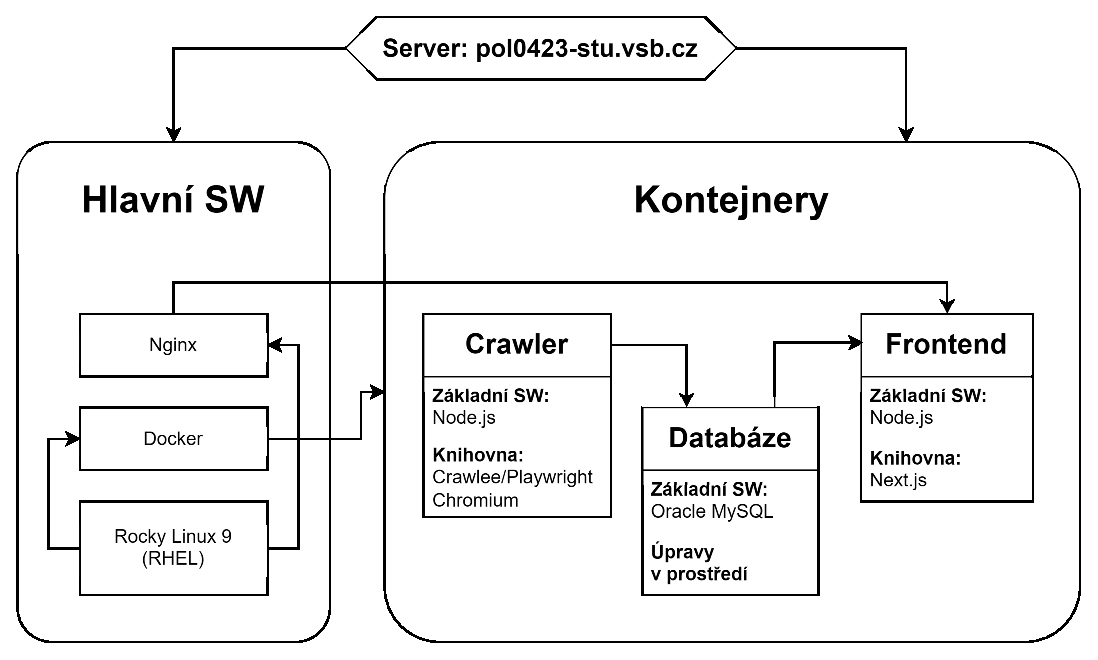
\includegraphics[width=0.75\linewidth]{Figures/structure.eps}
    \caption{Návrhový diagram technického řešení aplikace}
    \label{fig:structure-diagram}
\end{figure}

Jak můžete vidět na přiloženém diagramu v obrázku \ref{fig:structure-diagram}
na stránce \pageref{fig:structure-diagram}, návrh technického řešení
je rozdělen na hlavní software a kontejnerovou část, která obsahuje
3 kontejnery. Crawler a databáze jsou součástí backendu, který je pomocí
databáze propojen s frontendem.

Hlavním softwarem je operační systém \emph{Linux}, na němž běží
kontejnerizační SW \emph{Docker} a dále webserverový SW \emph{Nginx}.
Docker poskytuje prostředí pro 3 kontejnerizované služby:

\begin{itemize}
    \item \textbf{Crawler:} Aktivní část backendu, která periodicky
        prohledává weby čerpacích stanic a zjišťuje aktuální ceny
        pohonných hmot, které následně zapisuje do databáze.
    \item \textbf{Databáze:} pasivní část backendu, která uchovává
        zaznamenané informace o PHM (typ, kvalita, název, cena)
        daných ČS.
    \item \textbf{Frontend:} Uživatelské prostředí aplikace, které
        zprostředkovává uživateli grafické rozhraní, ve kterém může
        vyhledávat, řadit a filtrovat PHM a jejich ceny na základě
        geografické lokace a maximálního okruhu.
\end{itemize}

Webservový SW Nginx poskytuje reverse proxy pro snadný přístup ke službě
prostým zadáním domény do adresního řádku prohlížeče. Zamýšlené je použití
SSL pro HTTPS a přesměrování nezabezpečeného portu HTTP na zabezpečený port
HTTPS.

\section{Příprava operačního systému a konfigurace DNS}
\label{sec:os-preps-dns-config}

Jako operační systém serveru jsem zvolil Rocky Linux,
který mi byl doporučen administrátory školní sítě. Tato linuxová
distribuce je založena na RHEL. Součástí konfigurace VM je také
nastavení sítě. Neměnná IP adresa je získána z DHCP serveru,
avšak se jedná pouze o IPv4. IPv6 je potřeba nastavit ručně.
Pro server je předkonfigurovaný také DNS záznam pro IPv4 a IPv6,
který vypadá následovně:

\begin{verbatim}
Name                       Type   TTL   Section    IPAddress
----                       ----   ---   -------    ---------
pol0423-stu.vsb.cz         AAAA   7200  Answer     2001:718:1001:207::64
pol0423-stu.vsb.cz         A      7200  Answer     158.196.109.64
\end{verbatim}

DNS záznam AAAA je vazba na IPv6 adresu, zatímco DNS záznam A
je vazba na IPv4.

\subsection{Instalace OS a počáteční konfigurace sítě serveru}
\label{sec:os-installation-initial-server-network-config}

Server se nachází na VMware vSphere serveru, dostupný
na adrese vcs.vsb.cz. Prvním krokem byla instalace OS Rocky Linux,
která proběhla přes virtuální konzoli serveru. Instalační program
byl ve formě GUI, přes které jsem nastavil uživatelský účet správce
\texttt{marpolda}, nastavil jsem mu heslo a zapnul mu práva správce.
Účet správce \texttt{root} je vypnutý, lze ho tedy použít jen pomocí
příkazu \texttt{sudo}. Po instalaci OS byla dalším krokem instalace
nástrojů virtuálního stroje. Po neúspěšném pokusu v instalaci balíčku
VMware Tools jsem se rozhodl využít místo toho otevřený balíček
\texttt{open-vm-tools}. Pro práci s textovými soubory jsem si
také nainstaloval balíček \texttt{nano}, který poskytuje jednoduchý
textový editor přímo v příkazovém řádku.

Dalším krokem je nastavení IPv6 sítě. Jelikož IPv6 adresa není
DHCP serverem přidělena, je potřeba adresu nastavit ručně. Pro to
využijeme výše zmíněný DNS záznam pro IPv6 vazbu. Tento proces
je také zapotřebí provést pomocí virtuální konzole (viz listing
\ref{lst:net-modify} na stránce \pageref{lst:net-modify}).

Otestujeme konektivitu IPv4 a IPv6:

\begin{verbatim}
PS C:\Users\marpo> ping -4 pol0423-stu.vsb.cz

Pinging pol0423-stu.vsb.cz [158.196.109.64] with 32 bytes of data:
Reply from 158.196.109.64: bytes=32 time<1ms TTL=61
Reply from 158.196.109.64: bytes=32 time<1ms TTL=61
Reply from 158.196.109.64: bytes=32 time<1ms TTL=61
Reply from 158.196.109.64: bytes=32 time<1ms TTL=61

Ping statistics for 158.196.109.64:
    Packets: Sent = 4, Received = 4, Lost = 0 (0% loss),
Approximate round trip times in milli-seconds:
    Minimum = 0ms, Maximum = 0ms, Average = 0ms
PS C:\Users\marpo> ping -6 pol0423-stu.vsb.cz

Pinging pol0423-stu.vsb.cz [2001:718:1001:207::64] with 32 bytes of data:
Reply from 2001:718:1001:207::64: time=2ms
Reply from 2001:718:1001:207::64: time=1ms
Reply from 2001:718:1001:207::64: time<1ms
Reply from 2001:718:1001:207::64: time=1ms

Ping statistics for 2001:718:1001:207::64:
    Packets: Sent = 4, Received = 4, Lost = 0 (0% loss),
Approximate round trip times in milli-seconds:
    Minimum = 0ms, Maximum = 2ms, Average = 1ms
\end{verbatim}

Pro přístup na server pomocí SSH jsem si také importoval ručně
přes konzoli SSH klíče obou mých počítačů, které využívají kvantově
rezistentní algoritmus \texttt{ed25519}. Z důvodu bezpečnosti jsem
také provedl vypnutí přihlašování pomocí uživatelského hesla.
Tento krok jsem provedl vytvořením nového souboru
\texttt{/etc/ssh/sshd\_config.d/01-nopasswordlogin.conf}
s následujícím obsahem:

\newpage

\begin{verbatim}
#################################################
# Disable password logins
#################################################

PasswordAuthentication no
\end{verbatim}

Soubory v adresáři \texttt{/etc/ssh/sshd\_config.d} jsou automaticky
importovány v souboru\\
\texttt{/etc/ssh/sshd\_config}, který obsahuje konfiguraci SSH Daemon
serveru.

Následně stačilo restartovat službu SSH Daemon:

\begin{verbatim}
# systemctl restart sshd.service
\end{verbatim}

Přístup na server pomocí SSH jsem následně otestoval:
\begin{verbatim}
PS C:\Users\marpo> ssh marpolda@pol0423-stu.vsb.cz
The authenticity of host 'pol0423-stu.vsb.cz (158.196.109.64)' can't be established.
ED25519 key fingerprint is SHA256:oHy0UKZisrWxLKQtp5Xpezo53FNXZudKJ6/WVHeScI4.
This host key is known by the following other names/addresses:
    ~/.ssh/known_hosts:18: 158.196.109.64
Are you sure you want to continue connecting (yes/no/[fingerprint])? yes
Warning: Permanently added 'pol0423-stu.vsb.cz' (ED25519) to the list of known hosts.
Enter passphrase for key 'C:\Users\marpo/.ssh/id_ed25519':
Last login: Sat Mar  1 14:01:55 2025 from 158.196.52.150
[marpolda@pol0423-stu ~]$
\end{verbatim}

Z mého druhého počítače jsem se také úspěšně přihlásil:
\begin{verbatim}
[marpolda@archlinuxx-laptop ~]$ ssh pol0423-stu.vsb.cz
Enter passphrase for key '/home/marpolda/.ssh/id_ed25519':
Last login: Sun Mar  2 19:21:04 2025 from 2001:718:1001:698:99e2:f1ff:4e67:7618
[marpolda@pol0423-stu ~]$
\end{verbatim}

\section{Příprava kontejnerizace a instalace služeb}
\label{sec:containers-preps-services-install}

Nyní, když máme nastavený základní přístup, můžeme přistoupit
k instalaci softwaru pro kontejnerizaci a samotných kontejnerů
potřebných služeb. Pro kontejnerizaci jsem si vybral Docker,
který jsem nainstaloval z příslušného balíčku následovně:

\begin{verbatim}
# dnf install docker
\end{verbatim}

Dalším krokem je příprava samotných součástí aplikace. K tomu
jsem si vytvořil vývojové prostředí Gitu, ve kterém bude
probíhat vývoj aplikace a příprava pro její nasazení na server.
Toto prostředí se také nachází na GitHubu, kde je vidět
aktuální podoba této aplikace. Aplikaci jsem se rozhodl pojmenovat
\emph{PetrolScan}. Všechny součásti aplikace obsahují soubor
\texttt{Dockerfile}, který vytváří Docker obrázek dané součásti.
Všechny tyto součásti jsou pospojovány souborem \texttt{docker-compose.yml},
který součásti propojuje a vytváří tak ucelenou službu.

Vyvíjené součásti aplikace jsou:

\begin{itemize}
    \item Webová aplikace:
        \texttt{\url{https://github.com/POL0423/petrolscan-web-app}}
    \item Crawler:
        \texttt{\url{https://github.com/POL0423/petrolscan-crawler}}
    \item Docker Compose:
        \texttt{\url{https://github.com/POL0423/petrolscan-docker-compose}},
        Listing \ref{src:docker-compose.yml} na stránce
        \pageref{src:docker-compose.yml}
\end{itemize}

\subsection{Výběr softwaru pro crawler}
\label{sec:crawler-solutions}

Jako první jsem se rozhodl najít vhodné self-hosted webové crawlery
a scrapery. Crawlerům se v teorii věnuji v sekci \ref{sec:research-crawlers}
v kapitole \ref{ch:initial-research}
na stránce \pageref{sec:research-crawlers}. Na dotaz k vyhledávání
mi ChatGPT \cite{givNscvAOqB1nMpq} %Ref: GPTCrawlers
našel následující možnosti:

\begin{itemize}
    \item Crawlee
    \item Scrapy
    \item EasySpider
\end{itemize}

Rozhodl jsem se pro Crawlee.

\subsubsection{Zkouška Crawlee}
\label{sec:crawlee-trial}

Tento crawler funguje v Node.js, a nabízí jednoduchou instalaci pomocí
jednoduchého příkazu. Crawler simuluje procházení webu člověkem pomocí
bezhlavičkových webových prohlížečů, které jsou schopné také interpretovat
Javascriptový kód.

Zkušební test ukázkového crawleru proběhl v pořádku.
První pokus o spuštění neuspěl, neboť chyběly Playwright bezhlavičkové
prohlížeče. Po instalaci těchto prohlížečů se již crawler spustil.

Velmi příjemným zjištěním bylo, že builder již automaticky vygeneruje
soubor \texttt{Dockerfile}, pro crawler tak lze rovnou vytvořit
Docker image, který se jen posléze nahraje na Docker Hub a lze s ním
dále pracovat.

\subsubsection{Tvorba crawleru}
\label{sec:crawler-preps}

Nejprve je nutné prozkoumat webové stránky různých čerpacích stanic.
Uvažujme tak tyto čerpací stanice:

\begin{itemize}
    \item \textbf{Globus}
    \item Orlen
    \item Shell
    \item EuroOil
    \item \textbf{ONO}
    \item MOL
    \item OMV
    \item Prim
    \item Makro
\end{itemize}

Pro všechny tyto ČS tak je nutné prozkoumat a analyzovat jejich webové
stránky, abychom mohli z daných webových stránek vytáhnout příslušná data.
Začíná mravenčí práce, a sice prozkoumávání a analýza skladby jednotlivých
webových stránek ČS, zápis struktury každého webu a sestavení jednotlivých
šablon pro náš crawler tak, aby byl crawler schopen stránky procházet
a získávat daný obsah. Crawler tato data z webových stránek čte a zaznamenává
do databáze strukturovaně podle typu jednotlivých PHM, jejich značce
a umístění ČS.

\subsubsection{Globus}
\label{sec:preps-globus}

Tato ČS patří velkoobchodnímu řetězci (hypermarketu) stejného jména
a nachází se výhradně vždy v blízkosti prodejny. Globus lze v době
psaní této bakalářské práce najít jen v 16 různých městech a městských
částí v ČR:

\begin{itemize}
    \item Brno
    \item České Budějovice
    \item Chomutov
    \item Havířov
    \item Karlovy Vary ‒ Jenišov
    \item Liberec
    \item Olomouc
    \item Opava
    \item Ostrava
    \item Pardubice
    \item Plzeň ‒ Chotíkov
    \item Praha
    \begin{itemize}
        \item Čakovice
        \item Černý Most
        \item Štěrboholy
        \item Zličín
    \end{itemize}
    \item Trmice
\end{itemize}

Postup pro získání informací o cenách PHM z ČS je následující.

\begin{enumerate}
    \item Na webové stránce \url{www.globus.cz} klikneme na tlačítko s ikonou
        špendlíku. Pokud se nás web zeptá na výběr prodejny, zvolíme
        dle požadavků (například Ostravu). Pokud je zvolená prodejna
        nesprávná, lze výběr změnit kliknutím na tlačítko „Změnit“
        v prvním sloupci pop-up okénka.
    \item Požadované informace z této ČS jsou ve třetím sloupci (viz
        screenshot na obrázku \ref{fig:globus-cs} na stránce
        \pageref{fig:globus-cs}).
\end{enumerate}

Tento postup je potřeba automatizovat. K tomu nám právě poslouží již
zmíněný crawler. Každá ČS má jinou strukturu webu, a proto je potřeba
vytvořit pro každý web jeho vlastní crawler. K tomu lze využít threading
v Node.js.

\subsubsection{ONO}
\label{sec:preps-ono}

ČS ONO jsou v samostatné síti ČS provozované společností Tank ONO s.r.o.
Web se nachází na adrese \url{www.tank-ono.cz}, který je velmi jednoduchý
a přehledný. Postup k získání informací z ČS je následující:

\begin{enumerate}
    \item Načteme hlavní webovou stránku \url{www.tank-ono.cz}. Zobrazí
        se nám mapa s jednotlivými pobočkami sítě ČS ONO. Na této webové
        stránce se nachází celkem 43 stanic. Jejich mapu lze vidět
        na obrázku \ref{fig:tank-ono-mapa} na stránce
        \pageref{fig:tank-ono-mapa}. V tabulce \ref{tab:tank-ono-pobocky}
        na stránce \pageref{tab:tank-ono-pobocky} lze vidět jejich výčet.
    \item Kliknutím na jednu z položek v seznamu nebo kliknutím na pozici
        na mapě si lze zobrazit detail konkrétní ČS. Na obrázku
        \ref{fig:tank-ono-stranka} na stránce \pageref{fig:tank-ono-stranka}
        lze vidět strukturu webové stránky detailu ČS. Vlevo nahoře (a) je název
        a umístění ČS, zatímco vpravo dole je vidět tabulka PHM (b) včetně jejich
        cen v Kč (c) a eurech. Toto jsou data, která nás zajímají.
\end{enumerate}

\begin{table}[h]
    \centering
    \caption{Seznam ČS ONO}
    \label{tab:tank-ono-pobocky}
    \begin{tabular}{r l|r l}
        1.    & ČS Plzeň, Domažlická        & 24.   & ČS Sukorady u Mladé
                                                        Boleslavi\\
        2.    & ČS Nýřany                   & 25.   & ČS Podolí u Písku\\
        3.    & ČS Plzeň, Studentská        & 26.   & ČS Planá nad Lužnicí\\
        4.    & ČS Sokolov                  & 27.   & ČS Spytihněv\\
        5.    & ČS Teplice                  & 28.   & ČS Mošnov\\
        6.    & ČS Cheb                     & 29.   & ČS Kojetice-Tůmovka\\
        7.    & ČS Milovice u Hořic         & 30.   & ČS Cvikov\\
        8.    & ČS Chlumec                  & 31.   & ČS Chomutov - Přečaply\\
        9.    & ČS Jihlava                  & 32.   & ČS Zádveřice u Zlína\\
        10.   & ČS Trutnov                  & 33.   & ČS Brno-Popovice\\
        11.   & ČS Jindřichův Hradec        & 34.   & ČS Roudnice nad Labem\\
        12.   & ČS Vysoké Mýto              & 35.   & ČS Vysokov u Náchoda\\
        13.   & ČS Havraň                   & 36.   & ČS Praha - Štěrboholy\\
        14.   & ČS Kolaje u Poděbrad        & 37.   & ČS Řasnice-Strážný\\
        15.   & ČS Ústí n. L., Božtěšická   & 38.   & ČS Břest u Kroměříže\\
        16.   & ČS Praha, Dolní Měcholupy   & 39.   & ČS Vojtanov\\
        17.   & ČS Kbelnice                 & 40.   & ČS Dobkovice u Děčína\\
        18.   & ČS Havlovice u Domažlic     & 41.   & ČS Březno u Loun D7\\
        19.   & ČS Mělník                   & 42.   & ČS Brno-Hviezdoslavova\\
        20.   & ČS Krupá u Rakovníka        & 43.   & ČS Studénka - D1
                                                        exit 336\\
        21.   & ČS Dolní Dvořiště - ONO I   & 44.   & ČS Ostrov nad Ohří\\
        22.   & ČS Dolní Dvořiště - ONO II  & 45.   & ČS Chlumčany u Přeštic\\
        23.   & ČS Církvice u Kutné Hory
    \end{tabular}
\end{table}

\subsubsection{Vyřazené čerpací stanice}
\label{sec:preps-removed-stations}

Během analýzy zmíněných webů ČS jsem zjistil, že právě pouze Globus
a ONO poskytují ceny PHM. Následující weby řetězců ČS jsem musel
z projektu vyřadit, neboť nesplňují požadavky k dolování dat.

\begin{itemize}
    \item \textbf{OMV:} Tato síť ČS poskytuje ceny PHM ve formátu,
        který vyžaduje použití OCR čtečky, jejíž implementace
        by byla velmi náročná, a časově by nebylo reálné čtečku
        do projektu zakomponovat.
    \item \textbf{Orlen:} Webové stránky této ČS využívají REST API,
        což je vysoké plus. Ale to samo o sobě nestačí. Pokud ani
        v API, ani na webové stránce nejsou k dispozici ceny PHM,
        jen slevy na tankovací kartu či aplikaci této sítě, nelze
        tato data v porovnání cen PHM použít.
    \item \textbf{Shell, EuroOil, MOL a Prim:} Tyto ČS informace
        o cenách PHM na svých webových stránkách vůbec neposkytují,
        čímž nelze data z těchto webových stránek použít.
    \item \textbf{Makro:} Tato ČS sice ceny na webu uvádí, a to
        v přijatelném formátu, ale web implementuje pokročilé
        antiscraping mechanismy, které detekují a blokují crawlery
        podobné tomuto projektu. Z toho důvodu byl tento crawler
        během jeho vývoje vyřazen. Crawler zkrátka nemohl tyto
        mechanismy obejít a k implementaci protichůdných opatření
        již nezbýval dostatek času.
\end{itemize}

\subsubsection{Návrh strukturizace crawleru}
\label{sec:preps-crawler-structure}

Pro snazší vývoj a lepší údržbu aplikace je potřeba ji rozdělit na jednotlivé
části, které plní své specifické úlohy.

\begin{itemize}
    \item \textbf{Hlavní část:} Jedná se o hlavní spouštěcí kód, který volá
        další moduly.
    \item \textbf{Dílčí crawlery:} Tyto části provádějí samotnou sklizeň.
        Jedná se o samotnou implementaci logiky dílčích crawlerů. To jsou
        dva moduly: Globus a ONO. Oba tyto moduly mají společný nadřazený
        abstraktní modul, který definuje společné vlastnosti a metody
        těchto modulů.
    \item \textbf{Databázová spojka:} Tato část propojuje crawlery s databází
        a umožňuje jim do databáze zapisovat nasbíraná data.
    \item \textbf{Definice datových typů:} V této části definuji některé
        datové typy, které dílčí crawlery používají. Datové typy jsou
        definovány kvůli snadnější identifikaci a implementaci práce
        s informacemi.
    \item \textbf{Crontab:} Jedná se o skript, který periodicky každý den
        ve 3:00 spouští crawler a zajišťuje zapisování výstupu konzole
        do logovacího souboru.
\end{itemize}

\subsection{Databáze}
\label{sec:preps-db}

Databázím se podrobně věnuji v teoretickém rozboru
v sekci \ref{sec:research-db} kapitoly \ref{ch:initial-research}
na stránce \pageref{sec:research-db}.

Pokud je crawler mozkem aplikace, který vyhledává data a ukládá je,
pak databáze je určitě srdcem celé aplikace, protože umožňuje její fungování.
Bez databáze by aplikace fungovat nemohla. K dispozici je několik různých
softwarů. Především bych vyjmenoval následující možnosti:

\begin{itemize}
    \item \textbf{MySQL:} Zřejmě nejpoužívanější databázový software na světě.
        Jeho předností je jednoduché použití, všestrannost, a široká
        kompatibilita s různými softwary pro backend i frontend. MySQL
        je k dispozici ve více variantách:
        \begin{enumerate}
            \item \textbf{MySQL:} Originální verze MySQL, která je stále
                aktivně vyvíjená. Tuto verzi lze najít na většině komerčních
                serverů. Dnes vlastněná společností Oracle.
            \item \textbf{MariaDB:} Jedná se o fork originální verze MySQL
                (fork znamená, že se jedná o verzi odvozenou z původní).
                V dnešní době pro většinu menších projektů příjemná
                alternativa, která je zdarma a open-source.
        \end{enumerate}
    \item \textbf{PostgreSQL:} Rychlý a moderní nástupce MySQL. Tento
        databázový engine je nejvíce kompatibilní s moderními nástupci
        webové technologie (zejména Reactu, viz další podsekce), které
        v současnosti dominují internetu.
    \item \textbf{SQLite:} Jednoduchý a nenáročný databázový model určený
        pro lokální aplikace malé velikosti. Předností tohoto modelu
        je skutečnost, že běží přímo v dané aplikaci a nepotřebuje tedy
        zvlášť server pro správu dat. Nevýhodou je malá škálovatelnost.
\end{itemize}

Pro svou aplikaci jsem si vybral \textbf{MySQL}, jelikož poskytuje širokou
kompatibilitu, je jednoduchý k použití, všestranný a mám s ním již předchozí
zkušenost. Jedná se o průkopníka v moderních databázových systémech, který
vydláždil cestu jeho nástupcům. MySQL používá SQL pro komunikaci s aplikací,
což je strukturovaný dotazovací jazyk nápadně podobný angličtině.

\subsection{Frontend}
\label{sec:preps-frontend}

Podrobně se frontendům věnuji v teoretickém rozboru
v sekci \ref{sec:research-frontend} kapitoly \ref{ch:initial-research}
na stránce \pageref{sec:research-frontend}.

Frontend je tváří celé aplikace. Jedná se o tu část aplikace, kterou vidí
její uživatel. Tato část zpracovává data z databáze a zprostředkovává je
uživateli pro jeho další zpracování. Existuje mnoho webových technologií
založených na různých programovacích a značkovacích jazycích, které jsou
na internetu široce používané. Vyjmenoval bych zejména tyto nejpoužívanější:

\begin{itemize}
    \item \textbf{Statické HTML/CSS:} Jedná se čistě o statické webové
        stránky, tak jak jsou uložené na webovém serveru. Jednoduchým
        HTTP requestem si uživatel prostřednictvím webového prohlížeče
        zažádá stránku, webový server najde její odpovídající soubor,
        a obsah stránky zašle do počítače uživatele. Výhoda je extrémní
        jednoduchost, nevýhodou je, že nelze vytvářet složitější aplikace,
        které vyžadují určitou interaktivitu a případně nějaké složitější
        výpočty. Jedná se o první webovou technologii.
    \item \textbf{HTML/CSS s JS:} Malý upgrade z předchozí technologie,
        nyní obohacená o jednoduchou formu programování na webu. JavaScript
        nabízí možnosti, jak stránku doplnit o různé efekty a interaktivitu,
        a umožňuje jednoduché algoritmizační úkony. Výhodou je jednoduchost
        a jistá forma interaktivizace. Nevýhodou je fakt, že veškerý
        programový kód aplikace běží v počítači uživatele, a tak není možné
        pracovat s databází na serveru, aniž by došlo k úniku autentizačních
        údajů.
    \item \textbf{PHP:} Jedná se o doplňkový software v současnosti nejvíce
        využívaný společně s webovým serverem Apache a Nginx, a zároveň
        se jedná o programovací jazyk, ve kterém jsou psané webové aplikace.
        PHP může sloužit zároveň jako backend i frontend. Uživateli tento
        software posílá data nejčastěji ve formátu HTML/CSS/JS, ale může
        využívat i některé formáty serializovaných dat (např. XML nebo JSON),
        případně obrázkové, video či audio formáty. Výhodou je skutečnost,
        že tento software umožňuje část aplikace spouštět na serveru
        a uživatel tak uvidí konečný výstup, případně částečně zpracovaný
        výstup, se kterým lze posléze manipulovat na uživatelské straně.
        Nevýhodou je poměrně složitější a obtížnější serializace dat, která
        je způsobená zejména stářím standardu. V PHP existuje několik
        frameworků, ale jen jeden nejpoužívanější framework je univerzální
        pro širokou škálu různých projektů, které vyžadují vývoj vlastních
        funkcí: \textbf{Laravel}. Tento framework umožňuje tvorbu originální
        webové aplikace v PHP, kde jsou k dispozici vývojářské nástroje
        pro správu dat, jejich čtení, zápis a další zpracování. Nevýhodou
        tohoto frameworku je chybějící nástroje pro rychlý webdesign.
        Na druhou stranu však má vývojář volnou ruku ve volbě vlastního
        řešení.
    \item \textbf{Node.js:} Node.js lze úspěšně použít nejen pro backend,
        ale také i pro frontend. V kombinaci s dalšími frameworky, které
        umožňují jednodušší tvorbu webové aplikace, se jedná o moderní
        způsob poskytování webového obsahu. Toto jsou nejpoužívanější
        frameworky:
        \begin{itemize}
            \item \textbf{React:} Základní průkopník moderního webu.
                Jedná se o knihovnu, která položila základy moderního
                webu a vytvořila koncept webového serveru v JavaScriptu.
            \item \textbf{Next.js:} Moderní React framework vyvíjený
                společností Vercel. Výhodou je jednoduchost použití
                a nativní inkluze moderních CSS frameworků, jako např.
                Tailwind CSS nebo CSS Modules.
            \item \textbf{Vue.js:} Konkurenční framework oproti Next.js.
                Jedná se o progresivní framework, který poskytuje jednoduché
                vývojářské nástroje pro frontend.
            \item \textbf{Nuxt.js:} Odvozený z Vue.js, doplňuje jej
                o full-stack nástroje, lze jej tedy využít i jako backend.
        \end{itemize}
\end{itemize}

Pro mou aplikaci jsem se rozhodl využít Node.js s využitím frameworku Next.js.
S Node.js již mám nějaké předchozí zkušenosti, JavaScript je poměrně
jednoduchý programovací jazyk, z něj odvozený TypeScript navíc přidává
jednoduché zabezpečení aplikace z hlediska datových typů. Next.js se mi jeví
jako optimální volba, vzhledem k jednoduchosti a dostupnosti různých
předpřipravených nástrojů pro rychlý webový design.

\endinput

\chapter{Funkce vyvíjené aplikace}

\endinput

\chapter{Závěr}
\label{sec:conclusion}

Tvorba projektu byla poměrně náročná, nicméně velmi zajímavá.
Nejen, že~jsem využil něco z~toho, co již znám, ale~vyzkoušel jsem~si
i~něco nového, a~spoustu se~toho při~tvorbě této aplikace naučil.
Způsobů, jakým se~dají tvořit moderní webové stránky, je~nepřeberné
množství. Lze využít staré osvědčené metody, ale technologie a~trend
se~ubírají novým směrem a~posouvají~se kupředu. I~z~toho důvodu je~nutné
se~neustále vzdělávat a~držet krok s~dobou. Je to jedno z~mála, co~člověk
může udělat pro~to, aby~si~udržel přehled a~nezaostával za~ostatními.

Pokud bych měl zhodnotit splnění bodů, tak si~myslím, že~ačkoliv
se~při~rešerši a~vývoji vyskytly nečekané potíže, dokázal jsem~si s~nimi
poradit a~projekt dotáhnout zdárně do~úspěšného konce.

Musím zdůraznit jednu věc: Tento projekt je~pouze demonstrační.
Účelem bylo vyvinout webovou aplikaci, která pravidelně aktualizuje
ceny PHM, a~na~základě zadané geografické lokace je~porovnává, filtruje
a~nabízí uživateli. Pro~demonstraci byly nakonec vybrány 2~sítě čerpacích
stanic, ze~kterých jsou data získávána. Původním záměrem bylo sice použití
8~ČS (následně se~počet rozšířil na~9), ale při zkoumání dostupnosti dat
jsem zjistil, že~pouze 3~z~těchto čerpacích stanic nabízí data v~rozumném
formátu a~nakonec jsem zjistil během vývoje, že~jen 2~čerpací stanice
lze reálně použít. Problém by~nastal, kdyby dostupná byla jen 1~ČS.
Tím, že~dostupné jsou 2, je~porovnání cen možné. A~to~je základní předpoklad
k~funkční aplikaci porovnávače cen.

\begin{enumerate}
    \item \textbf{Motivace a~přehled podobných projektů.}
        
        Tato část zkoumá hnací impuls, který mě~vedl k~výběru tohoto
        tématu a~také podobné projekty, které jsou mému nápadu podobné.
        Popsal jsem tam webové stránky a~aplikace, které nabízí srovnání
        cen PHM na~ČS po~celé ČR nebo dokonce v~celé Evropě.

    \item \textbf{Technologie pro~návrh webových aplikací.}

        V~této části se~věnuji rozboru používaných technologií
        pro~návrh a~implementaci webových aplikací, kde~porovnávám
        jednotlivé knihovny a~frameworky, zhodnocuji jejich
        výhody a~nevýhody a~popisuji jejich typické využití.
        V~této části jsem využil umělé inteligence, konkrétně
        ChatGPT, k~rešerši. Tvrzení v~této kapitole jsou řádně
        citována, zdroj informací je~uveden jak z~ChatGPT, tak
        ze~zdrojů, které k~tvrzení umělá inteligence připojila.

    \item \textbf{Popis návrhu a~implementace.}

        Od~příprav, přes vývoj až~po~finální úpravy a~spuštění aplikace.
        Tato část popisuje postup tvorby jednotlivých dílčích součástí
        aplikace, jejich spojení, kontejnerizace a~následné finální
        spuštění na~VPS. Hlavním OS je~Rocky Linux, kde~je~nainstalován
        Nginx pro~provoz reverse proxy a~Docker, který obsahuje 3~kontejnery
        obsluhující jednotlivé části. Jeden kontejner je zaměřen
        na~databázi, další obsahuje crawler, který se~spouští periodicky
        každý den ve~3:00, a~poslední obsahuje webový frontend, který data
        z~databáze filtruje, řadí a~zobrazuje uživateli v~prohlížeči.
        Během vývoje aplikace jsem~si v~některých částech pomohl umělou
        inteligencí, konkrétně GitHub Copilotem, který mi~řešil obtížné
        chyby, jenž se~při~vývoji vyskytly, a~jejichž tradiční ladění
        by~znamenalo příliš velké prodloužení vývoje aplikace.

    \item \textbf{Zhodnocení dosažených výsledků.}

        Nebudu lhát, během vývoje došlo k~několika problémům, které
        finální podobu posunuly trochu jinak, než jsem původně očekával.
        Ve~všech případech si~však myslím, že~cíl bakalářské práce
        byl~splněn. Webová aplikace sice nevypadá tak, jak jsem si
        původně představoval, ale~základní funkcionalita byla dodržena.
        Crawler periodicky spouští procházení webu a aktualizuje databázi.
        Webový frontend nabízí uživateli možnost vyhledávání geografické
        lokace pomocí formuláře společně se~specifikací maximálního okruhu
        pro~porovnání, včetně možnosti změny řazení výsledků dle ceny
        (od~nejlevnějších nebo od~nejdražších) a~filtrování výsledků
        na~základě typu paliva či~jiného doplňkového produktu z~tankovacích
        stojanů či~jejich kvality. GUI webové aplikace je~sice minimální,
        ale~uživatelsky přívětivé a~přehledné.
\end{enumerate}

Ještě jednou pro~jistotu uvádím, že~jsem nad~rámec zadání bakalářské práce
po~dohodě s~vedoucím zařadil do~nabídky PHM k~porovnání také doplňkové
produkty dostupné z~tankovacích stojanů, které by~mohly řidiče zajímat.
Jedná~se zejména o~AdBlue (syntetickou močovinu) a~kapalinu do~ostřikovačů.
Tedy provozní kapaliny, které ze~své podstaty nejsou palivem, nicméně se~jedná
o~provozní kapaliny, které jsou nutné k~bezpečnému a~ekologickému provozu
automobilu.

Aplikaci by~samozřejmě šlo vylepšit a~případně přepracovat. Nabízí~se např.
využití umělé inteligence k~vyhledávání cen PHM a~dalších doplňkových
produktů a~služeb. Jiná možnost by~byla použití síly veřejnosti, která
by~mohla informace o~aktuálních cenách paliv a~doplňkových produktů a~služeb
doplňovat. Pokud jde o~prezentaci výsledků vyhledávání, tak více možností
pro~řazení, filtrování podle více typů a~kvalit produktů, apod. Geografické
určení uživatele by~mohlo případně probíhat i~geolokační službou prohlížeče.
Všechny tyto funkce jsou však již nad~rámec zadání této bakalářské práce
a~nejsou nezbytně nutné ke~splnění základních požadavků. Tyto možnosti však
lze nechat otevřené pro~případný výzkum v~rámci navazujícího studia
v~diplomové práci.

\endinput


% Seznam literatury
\printbibliography[title={Literatura}, heading=bibintoc]

% Prilohy
\appendix
\chapter{Ukázky webů ČS}

\begin{sidewaysfigure}
    \centering
    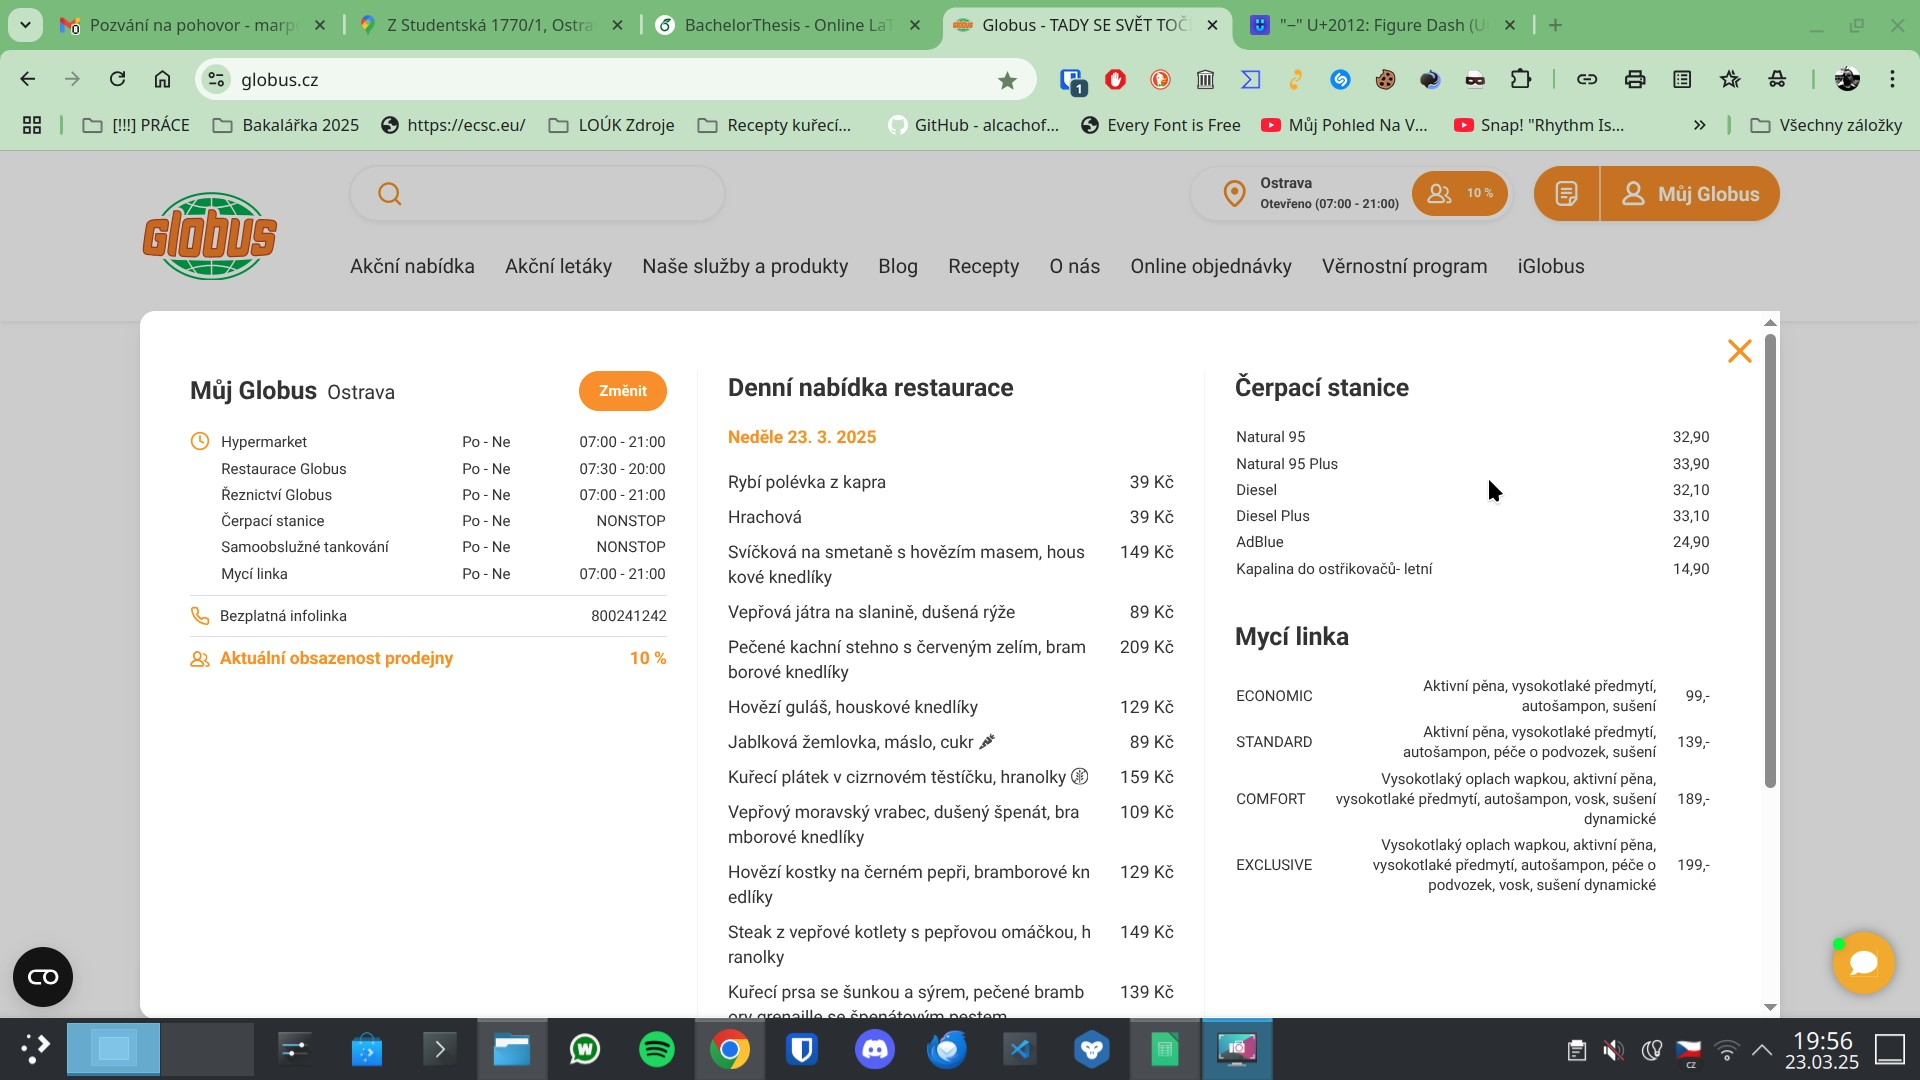
\includegraphics[width=\textwidth]{Figures/globus_vyber.jpg}
    \caption{Základní informace o prodejně Globus, včetně cen PHM
        přidružené ČS \cite{RlWZWiUaWElVCBZM}}
    \label{fig:globus-cs}
\end{sidewaysfigure}

\begin{figure}
    \centering
    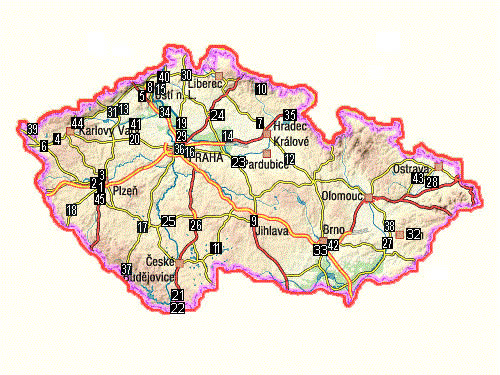
\includegraphics[width=\textwidth]{Figures/map_pump.jpg}
    \caption{Mapa čerpacích stanic ONO \cite{9n9VUsIjBwGy4lUb}}
    \label{fig:tank-ono-mapa}
\end{figure}

\begin{sidewaysfigure}
    \centering
    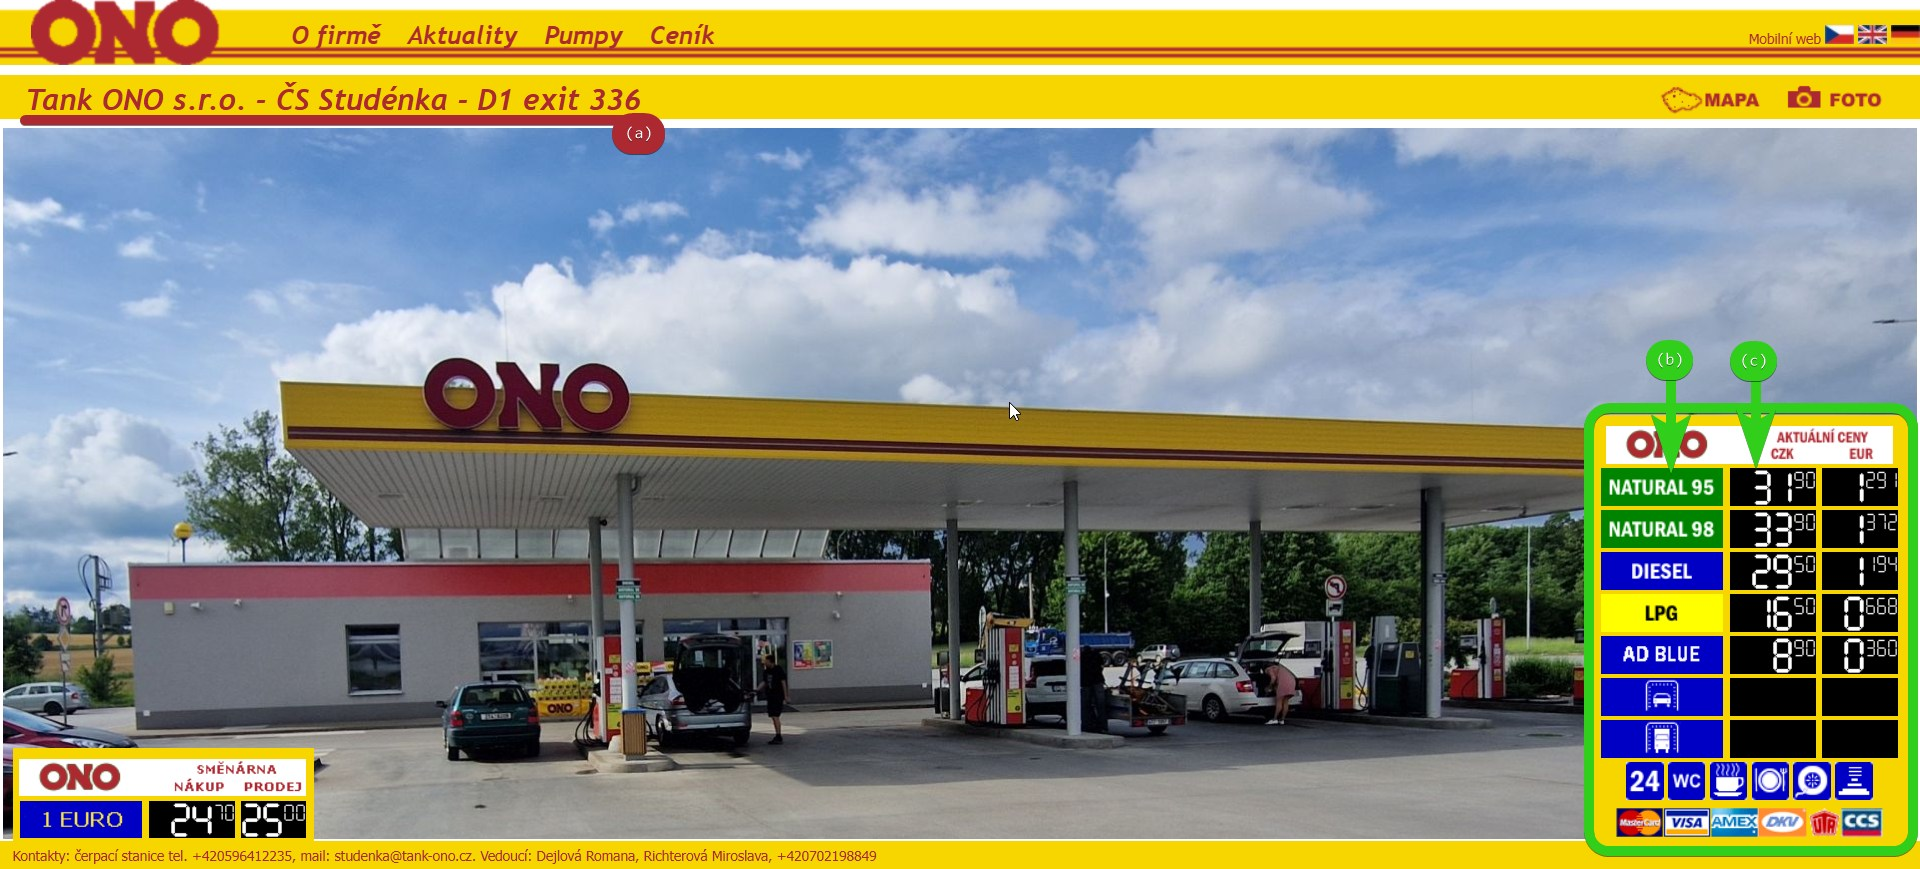
\includegraphics[width=\textwidth]{Figures/tank-ono-cs.jpg}
    \caption{Webová stránka s detailem ČS ONO
        \cite{9n9VUsIjBwGy4lUb}}
    \label{fig:tank-ono-stranka}
\end{sidewaysfigure}

\endinput

%\chapter{Instalace serveru a vývoj aplikace}

\begin{sidewaysfigure}
    \centering
    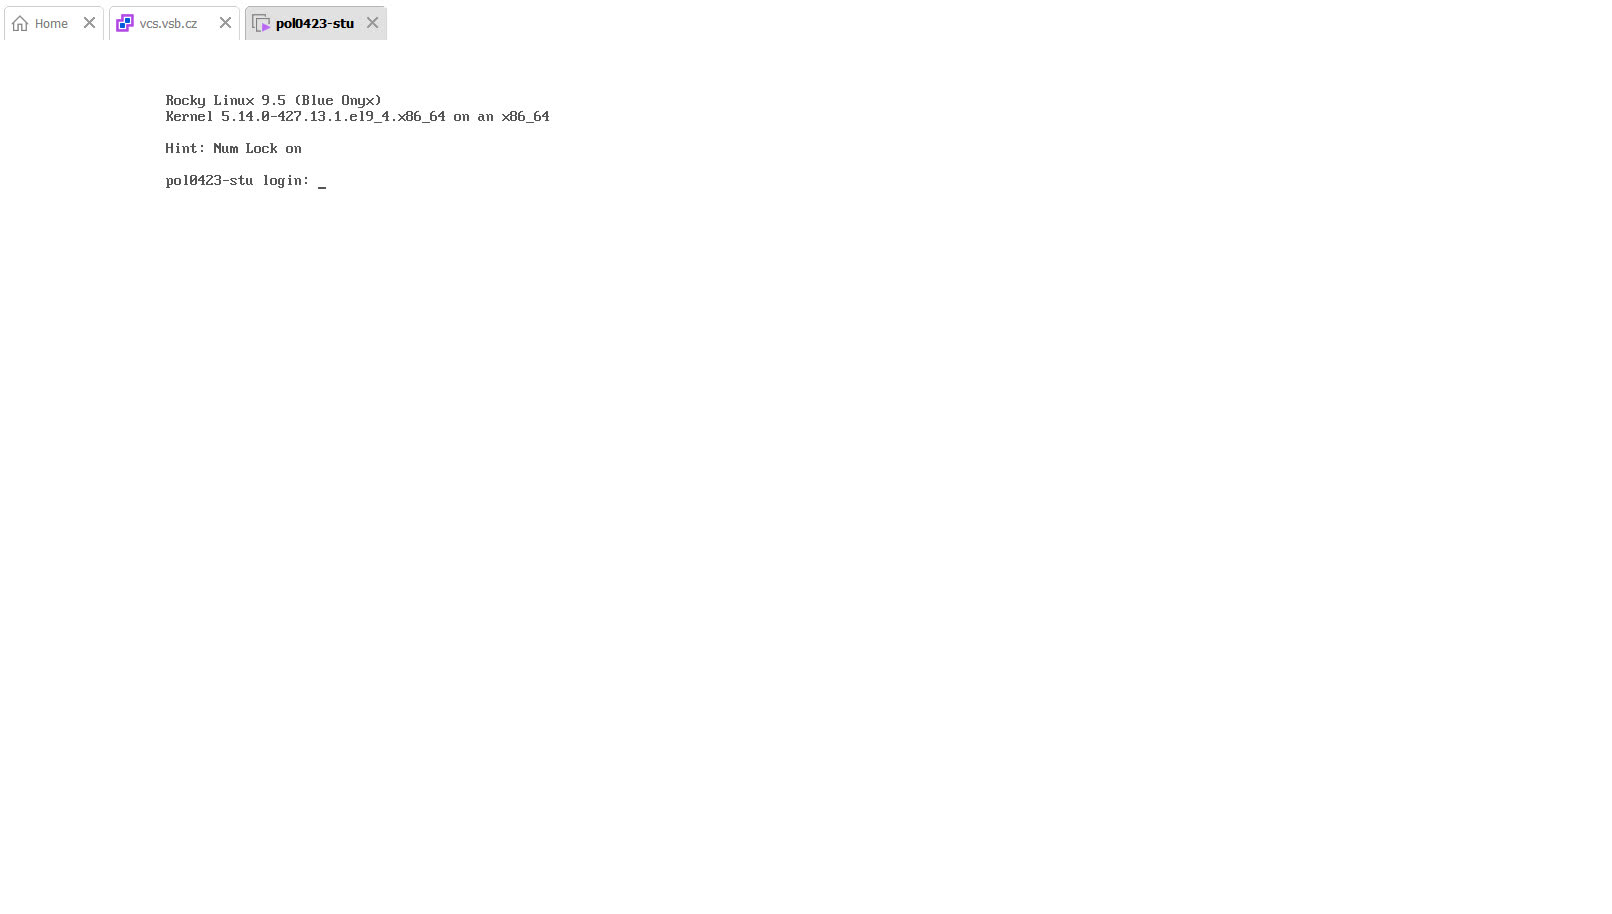
\includegraphics[width=\textwidth]{Figures/vmware_console.jpg}
    \caption{Konzole virtuálního serveru ve VMware Workstation Pro}
    \label{fig:vmware-workstation-pro}
\end{sidewaysfigure}

\newpage

\lstinputlisting[label=src:docker-compose.yml,caption={Soubor \texttt{docker-compose.yml} k sestavení Docker kontejnerů}]{SourceCodes/docker-compose.yml}

\begin{figure}
    \centering
    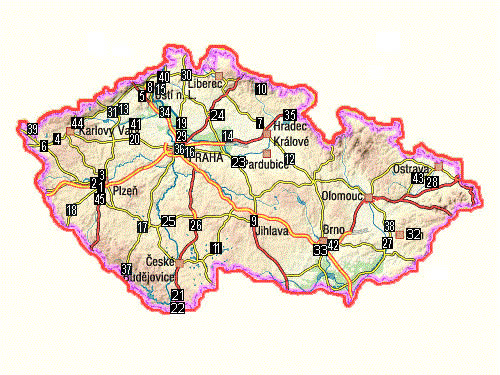
\includegraphics[width=\textwidth]{Figures/map_pump.jpg}
    \caption{Mapa čerpacích stanic ONO}
    \label{fig:tank-ono-mapa}
\end{figure}

\begin{sidewaysfigure}
    \centering
    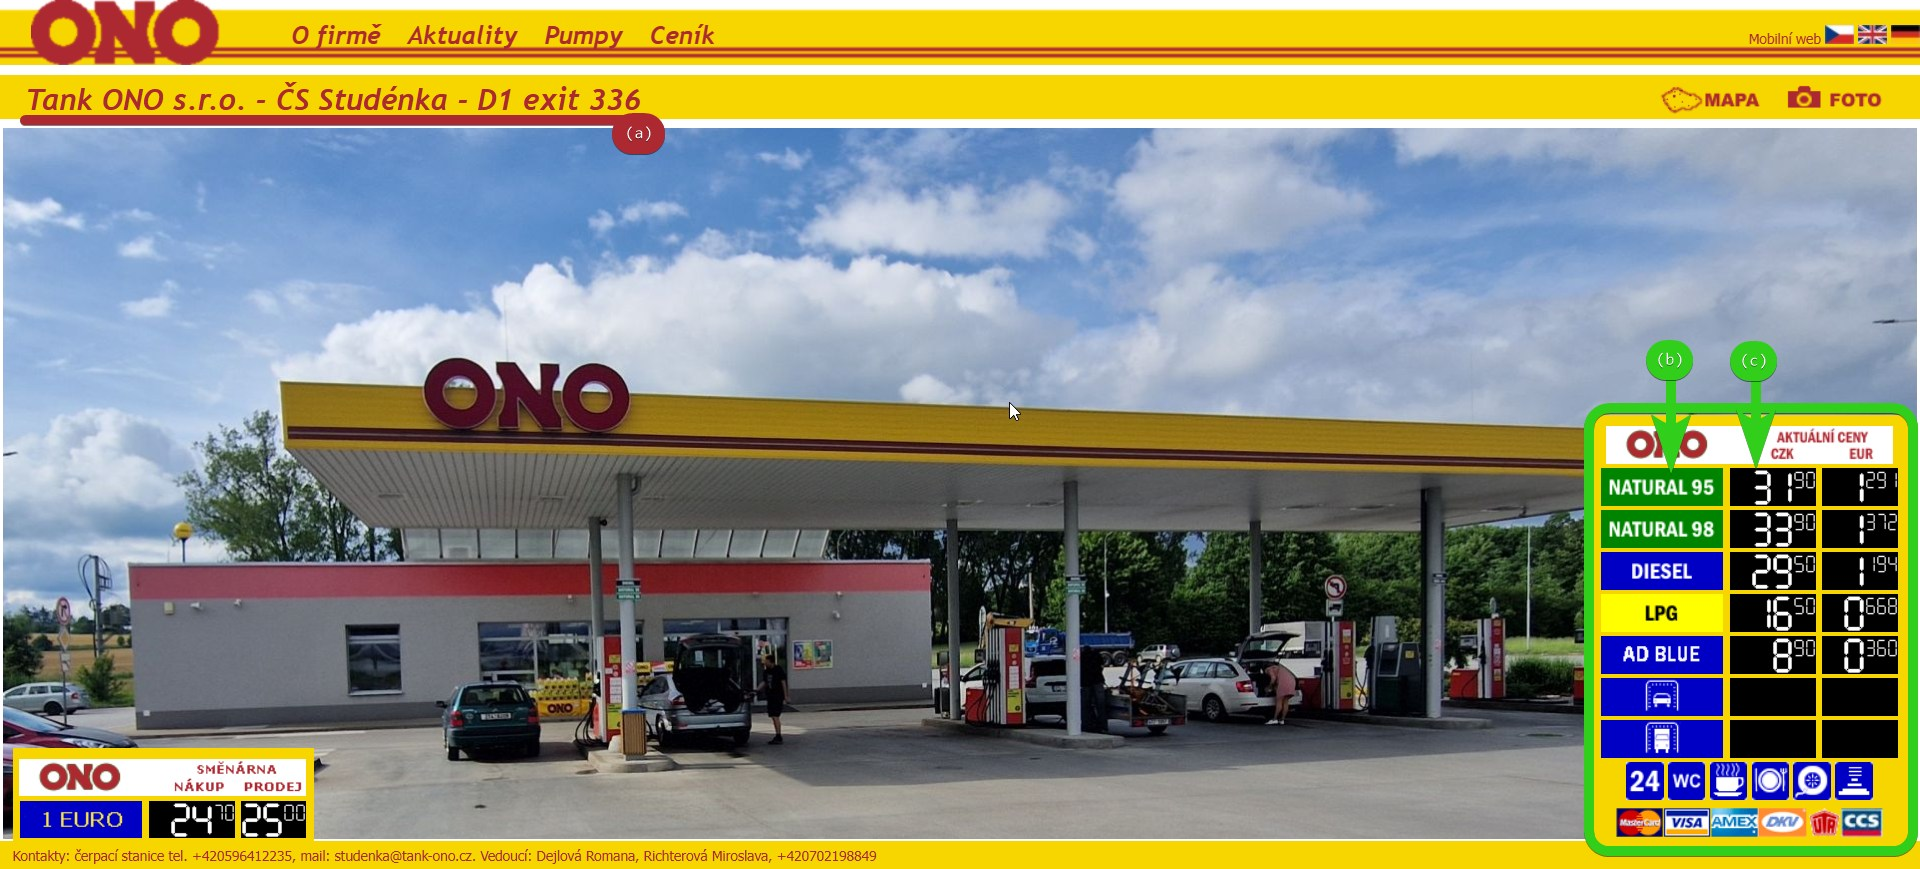
\includegraphics[width=\textwidth]{Figures/tank-ono-cs.jpg}
    \caption{Webová stránka s detailem ČS}
    \label{fig:tank-ono-stranka}
\end{sidewaysfigure}

% Priloha vlozena primo do hlavniho LaTeX souboru. Ne vsechny prilohy je nutne mit ve zvlastnich souborech.
%\chapter{Dlouhý zdrojový kód}
%\lstinputlisting[label=src:CppExternal,caption={Dlouhý zdrojový kód v jazyce C++ načtený s externího souboru}]{SourceCodes/ArraySortingAlgorithms.cpp}

\end{document}
